% nevpt2.tex -- SC- and PC-NEVPT2, their quasidegenerate (QD) extensions,
% analytic nuclear gradients, single-state analytic nuclear Hessians and
% nonadiabatic couplings, as implemented in free-breakfast's src/nevpt2 layer
% and the src/hessian calls built on it.
%
% This is a description of the code as it stands (7 November 2026, main at
% 862d9e0c), with the equations it evaluates and the algorithms it runs. The
% module READMEs under src/nevpt2/ and src/hessian/ are the finer-grained
% record (layouts, memory, every measured number); where the two disagree,
% the code and its READMEs win.
%
% Build: pdflatex nevpt2.tex, twice (cross-references).
\documentclass[11pt]{article}

\usepackage[T1]{fontenc}
\usepackage{lmodern}
\usepackage{microtype}
\usepackage[margin=2.5cm]{geometry}
\usepackage{amsmath,amssymb}
\usepackage{booktabs}
\usepackage{tabularx}
\usepackage{algorithm}
\usepackage[noend]{algpseudocode}
\usepackage[hidelinks]{hyperref}
\usepackage{tikz}
\usetikzlibrary{positioning,fit,backgrounds,arrows.meta,calc}

\tikzset{
  fn/.style={draw=black!70, rounded corners=2pt, align=center,
    font=\scriptsize, inner sep=2.5pt, minimum height=7mm,
    text width=#1, fill=white},
  fn/.default=3.3cm,
  entry/.style={fn=#1, draw=blue!60!black, very thick, fill=blue!8},
  entry/.default=3.3cm,
  hot/.style={fn=#1, draw=orange!70!black, thick, fill=orange!10},
  hot/.default=3.3cm,
  data/.style={draw=black!50, align=center, font=\scriptsize,
    inner sep=3pt, minimum height=7mm, text width=#1, fill=black!6},
  data/.default=3.3cm,
  group/.style={draw=black!45, dashed, rounded corners=4pt, inner sep=7pt},
  grouplabel/.style={font=\scriptsize\itshape, anchor=north west,
    inner sep=2pt},
  arr/.style={-{Stealth[length=1.8mm]}, black!75},
  side/.style={arr, dashed},
  edgelabel/.style={font=\tiny, fill=white, inner sep=1pt},
}

\newcommand{\code}[1]{\texttt{#1}}
\newcommand{\Lag}{\mathcal L}
\newcommand{\doi}[1]{\href{https://doi.org/#1}{doi:\nolinkurl{#1}}}
\newcommand{\G}[1]{\Gamma^{(#1)}}
\newcommand{\eps}{\varepsilon}
\newcommand{\Ecas}{E_{\mathrm{CAS}}}
\newcommand{\Ecorr}{E_{\mathrm{corr}}}
\newcommand{\heff}{h^{\mathrm{eff}}}
\newcommand{\Heff}{H^{\mathrm{eff}}}
\newcommand{\hb}{\bar h}
\newcommand{\Lb}{\Lambda}
\newcommand{\T}{\mathsf T}
\newcommand{\tr}{\operatorname{tr}}
\newcommand{\sym}{\operatorname{sym}}
\newcommand{\Tc}{\mathcal T}
\algrenewcommand\algorithmicrequire{\textbf{Input:}}
\algrenewcommand\algorithmicensure{\textbf{Output:}}

\title{SC- and PC-NEVPT2 and QD-NEVPT2 in free-breakfast\\
\large Energies, analytic nuclear gradients and Hessians, and nonadiabatic
couplings, density-fitted, on the GPU}
\author{free-breakfast implementation notes}
\date{7 November 2026}

\begin{document}
\sloppy
\maketitle

\begin{abstract}
This document describes the \code{src/nevpt2} layer of free-breakfast: the
strongly contracted (SC) and partially contracted (PC) $n$-electron valence
state perturbation theory (NEVPT2) energies of a CASSCF reference, their
quasidegenerate (QD) effective Hamiltonians over a state-averaged CASSCF,
the analytic nuclear gradient of every one of them, the analytic nuclear
Hessian of single-state SC and PC, the QD interstate
coupling and derivative (nonadiabatic) coupling, and what a QD
minimum-energy conical intersection search needs. Everything is density
fitted and runs on the device. The organising idea is that every
correlation quantity is a function of only three objects, the MO
one-electron matrix $h$, the fitted three-index tensor $B$ and the CI
vectors, so one reverse pass through the energy gives its adjoints
$(\hb, \Lb, \bar y)$, and from there each derivative is the CASSCF
machinery the tree already has: one Z-vector solve over the CI-relaxed
Hessian and one or two passes of the density-fitted derivative integrals.
The Hessian is the same idea one order up: the energy's tangent along each
coordinate's first-order response, forward over the reverse pass, against
$3N$ CP-CASSCF responses and the gradient's own multipliers.
No derivative is written by hand beyond a few scalar finishes, and no
finite difference appears in any production path except those that are
exact: the Hessian-vector products' bars at fixed multipliers are
polynomials of degree at most five along a line, and three symmetric
differences recover their derivative with no truncation error.
\end{abstract}

\tableofcontents

%======================================================================
\section{Scope and layering}
\label{sec:scope}

\paragraph{What is implemented.}
\begin{itemize}
\item SC- and PC-NEVPT2 class energies of one root
  \cite{angeli2001,angeli2001cpl,angeli2002}, over a Dyall zeroth-order
  Hamiltonian \cite{dyall1995}.
\item SC- and PC-QD-NEVPT2 \cite{angeli2004}: the effective Hamiltonian of
  $n$ roots of a state-averaged CASSCF, in the ``SA-NEVPT2'' scheme of
  Park \cite{park2020} (one set of orbitals, core and virtuals canonical
  over the state-averaged Fock), symmetrised and diagonalised.
\item Analytic nuclear gradients of single-state SC and PC-NEVPT2 on a
  single-state DF-CASSCF \cite{park2019,park2019arxiv}, and of any SC- or
  PC-QD-NEVPT2 state on a DF-SA-CASSCF at any weights \cite{park2020}.
\item Analytic nuclear Hessians of single-state SC- and PC-NEVPT2 on a
  single-state DF-CASSCF, all-electron, in Cartesian or caller-given
  coordinates (\S\ref{sec:hessian}), with the refusals that keep a
  non-smooth surface from being reported as a Hessian. Unpublished for any
  internally contracted MRPT2 as far as we know. There is no QD-NEVPT2
  Hessian.
\item The QD interstate coupling $\mathbf h_{PQ}$, and the full derivative
  coupling $\mathbf d_{PQ} = \langle\Psi_P|\nabla\Psi_Q\rangle$, including the
  PT2 term \cite{park2020,park2017}.
\item For conical-intersection searches: $\mathbf g_P$, $\mathbf g_Q$ and
  $\mathbf h_{PQ}$ at one set of $\Heff$ eigenvectors with no refusal of a
  degenerate pair, and bounds on how far the pair's gap moves when the
  SA-CASSCF is not fully converged; for PC, the mean gradient alone inside a
  degenerate CASSCF pair, where the branching plane has no limit.
\end{itemize}

\paragraph{Layering.} \code{src/nevpt2} sits over \code{core},
\code{integrals} (the density-fitted MO transform), \code{ci} (the strings,
sigma vectors and RDMs) and, for derivatives, \code{response} and
\code{mcscf} (the CASSCF Fock, CI-relaxed Hessian and Z-vector in
\code{response}; the DF gradient, derivative integrals and CASSCF couplings
in \code{mcscf}). It never imports \code{pipeline} or \code{hessian}. The
nuclear Hessian is assembled one layer up, in \code{hessian}
(\code{df\_sc\_nevpt2}, \code{df\_pc\_nevpt2}), from this layer's tangents
and Hessian-vector products and the CASSCF Hessian's parts. The pipeline's
\code{[nevpt2]}, \code{[nevpt2\_gradient]}, \code{[nevpt2\_nac]},
\code{[optimize]} and \code{[hessian]} steps wrap both. Its six sub-modules are:

\begin{center}
\small
\begin{tabularx}{\linewidth}{@{}lX@{}}
\toprule
module & role \\
\midrule
\code{nevpt2.density\_fitting} & MO blocks of $B$, the active $(tu|vw)$, the ten external blocks slab by slab, and their adjoints onto $\Lb$ (\S\ref{sec:df}) \\
\code{nevpt2.rdm} & dm3 and the integral-contracted 4-RDMs f3ca, f3ac, of one vector or between two, and their adjoints (\S\ref{sec:rdm}) \\
\code{nevpt2.energy} & the eight SC and PC class energies, the SC- and PC-QD effective Hamiltonians, the amplitude hand-over, the reverse passes of all four, and the single-state classes' forward tangents and Hessian-vector products (\S\S\ref{sec:energy}--\ref{sec:reverse}, \S\ref{sec:hvp}) \\
\code{nevpt2.gradient} & the energy as a function of $(h, B, C, c)$, $z^c$, the Lagrangians, Z-vectors and nuclear terms; single-state and QD, SC and PC (\S\S\ref{sec:ssgrad}--\ref{sec:qdgrad}); the builders' forward tangent and the Hessian-vector product in $(h, B, c)$ (\S\ref{sec:hessian}) \\
\code{nevpt2.nac} & the PT2 transition density and the QD derivative coupling (\S\ref{sec:nac}) \\
\code{nevpt2.intersection} & a QD pair's branching space and gap sensitivities (\S\ref{sec:meci}) \\
\bottomrule
\end{tabularx}
\end{center}

\paragraph{Provenance.} The energy kernels are a port of the
nevpt2-gpu-demo, itself a transcription of PySCF's \code{mrpt.nevpt2}
\cite{pyscf2020}: every einsum keeps the reference's subscripts, so the two
read side by side. The PC energy is validated against block2's
\code{WickICNEVPT2} \cite{block2}. The derivative layers are this tree's own.
A related device-resident approach, DMRG-QD-SC-NEVPT2 gradients and
couplings as one reverse-mode transpose of a contraction graph, is
Ref.~\cite{guerrero2026}.

%======================================================================
\section{Notation}
\label{sec:notation}

\paragraph{Orbitals.} $C$ ($n_{\mathrm{ao}}\times n_{\mathrm{mo}}$) maps AOs
$\mu,\nu$ to MOs, ordered core, active, virtual. Core (inactive) labels are
$i,j,k,l$, active $t,u,v,w$ (and $p,q,r,s$ inside active-only tensors),
virtual $a,b$ (and $r,s$ as the external labels of a class), general
$x,y,z$. Counts are $n_c$, $n_a$, $n_v$, $n_{\mathrm{mo}}$. A rotation is
$C \to C e^{\kappa}$, $\kappa$ real antisymmetric.

\paragraph{Integrals.} $h = C^\T h^{\mathrm{AO}} C$. With three-centre
integrals $(\mu\nu|P)$ and the Coulomb metric $(P|Q) = LL^\T$,
\begin{equation}
  B^{L}_{xy} = \sum_P (L^{-1})_{LP}\,\bigl(C^\T (\cdot\cdot|P)\, C\bigr)_{xy},\qquad
  (xy|zw) = \sum_L B^L_{xy} B^L_{zw},
  \label{eq:B}
\end{equation}
the density-fitting approximation \cite{vahtras1993}. Every two-electron
quantity below is built from $B$ through such products.

\paragraph{Densities.} Spin-summed $E_{xy}$; active RDMs
$\G1_{tu} = \langle E_{tu}\rangle$, dm2 $= \langle E_{tu}E_{vw}\rangle$, dm3
$= \langle E_{tu}E_{vw}E_{xy}\rangle$, in PySCF's unreordered layout. Between
a bra $\langle M|$ and a ket $|N\rangle$, $\gamma^{(MN)}_{tu} =
\langle M|E_{tu}|N\rangle$ and so on, unsymmetrised.

\paragraph{Fock matrices.} The inactive Fock and the generalised Fock are
\begin{equation}
  F^I_{xy} = \heff_{xy} = h_{xy} + \sum_j\bigl[2(xy|jj) - (xj|jy)\bigr],\qquad
  f_{xy} = F^I_{xy} + \sum_{tu}\gamma_{tu}\bigl[(xy|tu) - \tfrac12(xt|uy)\bigr],
  \label{eq:fock}
\end{equation}
and the orbital energies are $\eps_x = f_{xx}$ for $x$ core or virtual. On a
state average $\gamma \to \gamma^{\mathrm{SA}} = \sum_r w_r\G1_r$.

%======================================================================
\section{NEVPT2 and QD-NEVPT2}
\label{sec:theory}

\subsection{The zeroth-order Hamiltonian and the classes}

NEVPT2 partitions $H = H^{(0)} + V$ with Dyall's Hamiltonian
\cite{dyall1995}
\begin{equation}
  H^D = \sum_i \eps_i E_{ii} + \sum_a \eps_a E_{aa}
      + \sum_{tu}\heff_{tu}E_{tu}
      + \tfrac12\sum_{tuvw}(tu|vw)\bigl(E_{tu}E_{vw} - \delta_{uv}E_{tw}\bigr) + C,
  \label{eq:dyall}
\end{equation}
and splits the perturbation into eight classes $V^{(k)}_l$ by how many
electrons the active space gains ($k$) and from which external orbitals
($l$) \cite{angeli2001}. Their PySCF names are used throughout:

\begin{center}
\small
\begin{tabular}{@{}llll@{}}
\toprule
name & space & external tuple & $\Delta$ (orbital-energy part of the denominator) \\
\midrule
Sr     & $S^{(-1)}_r$   & $a$ & $\eps_a$ \\
Si     & $S^{(+1)}_i$   & $i$ & $-\eps_i$ \\
Sijrs  & $S^{(0)}_{ijab}$ & $(i,j,a,b)$ & $\eps_a + \eps_b - \eps_i - \eps_j$ \\
Sijr   & $S^{(+1)}_{ija}$ & $(i,j,a)$ & $\eps_a - \eps_i - \eps_j$ \\
Srsi   & $S^{(-1)}_{abi}$ & $(a,b,i)$ & $\eps_a + \eps_b - \eps_i$ \\
Srs    & $S^{(-2)}_{ab}$  & $(a,b)$ & $\eps_a + \eps_b$ \\
Sij    & $S^{(+2)}_{ij}$  & $(i,j)$ & $-\eps_i - \eps_j$ \\
Sir    & $S^{(0)}_{ia}$   & $(i,a)$ & $\eps_a - \eps_i$ \\
\bottomrule
\end{tabular}
\end{center}

Every class but Sijrs has active indices; Sijrs reads no RDM.

\subsection{The SC energy}

In SC-NEVPT2 each external tuple $t$ has one perturber, $P_t V|\Psi_0\rangle$.
Its norm $N_t = \langle\Psi_0|V^\dagger P_t V|\Psi_0\rangle$ and its Dyall
element $H_t$ (the active part of $\langle P_t V\Psi_0|H^D - E_0|P_t V\Psi_0\rangle$)
are quadratic forms of a slab row of integrals over RDM-built matrices, and
\begin{equation}
  E^{\mathrm{SC}} = \sum_{k}\sum_{t\in k} E_t,\qquad
  E_t = -\frac{N_t}{\Delta_t + H_t/N_t},
  \label{eq:sc}
\end{equation}
over the perturbers with $|N_t| > 10^{-14}$ (PySCF's \code{\_norm\_to\_energy}
guard; Sijrs and the one-function classes below have none). The matrices are the metrics (dm3, dm2, dm1 and
their hole forms) and the Dyall blocks \code{a16}, \code{a22}, \ldots{} of
PySCF, which for Sr and Si read the 4-RDM only through f3ca and f3ac
(\S\ref{sec:rdm}).

\paragraph{One-function classes (\#949).} Srs at two active electrons and Sij
at two active holes span one function per perturber: removing both electrons
leaves the active vacuum (filling both holes, the closed shell), so
$N_t \propto A_t^2$ for one amplitude $A_t = \sum_{pq}W_{pq}\langle\mathrm{vac}|
a_qa_p|\Psi\rangle$ and $H_t = \eta N_t$, $\eta$ that function's Dyall
energy, one number per state and class. Every CAS(2,2) has both. PySCF's
guard drops such a perturber wherever $A_t$, a smooth signed function of the
geometry, passes through zero, yet its QD couplings $T^t_{IJ} \propto
A^I_tA^J_t$ are linear in $A_t$ there: that was a $3$--$6\times10^{-8}\,E_h$/bohr
SC-QD gradient miss at ethylene's Py (\#894). So a one-function class (told by
$\tr\,\mathrm{dm1}$: Srs at 2, Sij at $2n_a - 2$) keeps every perturber,
with $c_t = -1/(\Delta_t + \eta)$ and
\begin{equation}
  \eta = \frac{\langle X, Y\rangle}{\langle Y, Y\rangle},
  \label{eq:eta}
\end{equation}
$X$ the class's Dyall block (a7, a9) and $Y$ its metric (rm2, hdm2) in the
pairing the $H$ and norm einsums contract. On a state's own RDMs $X = \eta Y$
to $10^{-15}$, so $\eta$ is every perturber's $H_t/N_t$ read with no
division by a small $N_t$. Off that structure (a raw direction in a test)
$\eta$ is the least-squares ratio, one smooth function that every pass
differentiates exactly. PC has no guard and is unchanged.

\subsection{The PC energy}

PC-NEVPT2 keeps the span of each class's internal functions
\cite{angeli2002}. For a class with metric $S$, Dyall matrix $K$, one-body
metric $S_1$ and a coupling factor $c$, a tuple's slab row $x_t$ and its
one-body row $h_t$ give
\begin{equation}
  E_t = -c\, b_t^\T (K + \Delta_t S)^{+} b_t,\qquad
  b_t = S x_t + S_1 h_t,
  \label{eq:pc}
\end{equation}
$(\cdot)^+$ the inverse on the span of $S$ that the metric cut keeps. $S$,
$K$ and $S_1$ are the same matrices SC builds (SC contracts each against one
row; PC solves with them), so PC is ``SC without the final contraction'':

\begin{center}
\small
\begin{tabular}{@{}llllll@{}}
\toprule
class & basis, $d$ & $S$ & $K$ & $S_1$ & $c$ \\
\midrule
Sr   & $(p,q,r)$, $n_a^3$ & dm3$[r,p,q,b,a,c]$ & a16 & dm2$[r,p,q,a]$ & 1 \\
Si   & $(p,q,r)$, $n_a^3$ & dm3\_h$[r,p,q,b,a,c]$ & a22 & dm2\_h$[r,p,q,a]$ & 1 \\
Sijr & $p$, $n_a$ & hdm1 & a3 & --- & $2\,$direct$-$exchange \\
Srsi & $p$, $n_a$ & dm1 & k27 & --- & $2\,$direct$-$exchange \\
Srs  & $(p,q)$, $n_a^2$ & rm2$[p,q,b,a]$ & a7 & --- & $\tfrac12$ \\
Sij  & $(p,q)$, $n_a^2$ & hdm2 & a9 & --- & $\tfrac12$ \\
Sir  & $(p,q)\oplus(p,q)$, $2n_a^2$ & spin-coupling blocks & a12, a13 & $[2\,\mathrm{dm1};\,-\mathrm{dm1}]$ & 1 \\
Sijrs & none & --- & --- & --- & SC's \\
\bottomrule
\end{tabular}
\end{center}

\subsection{QD-NEVPT2}

Over $n$ roots $|M\rangle$ of a state-averaged CASSCF sharing one set of
orbitals, with $\eps$ from $f^{\mathrm{SA}}$ for every root
(Zaitsevskii--Malrieu multipartitioning \cite{zaitsevskii1995},
Park's SA-NEVPT2 scheme \cite{park2020}), each root has its own perturber
space and Dyall Hamiltonian, and the couplings are
$C_{MN} = \langle M|V|\Psi^{(1)}_N\rangle$. With $\Psi^{(1)}_N$ the ket's
first-order function:
\begin{align}
  \text{SC:}\quad C_{MN} &= -\sum_t \frac{\bar T^t_{MN}}{\Delta_t + H^N_t/N^N_t},
  \qquad \bar T^t_{MN} = \tfrac12\bigl(T^t_{MN} + T^t_{NM}\bigr),
  \label{eq:qd-sc}\\
  \text{PC:}\quad C_{MN} &= -c\sum_t b^{M\leftarrow N\,\T}_t
    \bigl(K_N + \Delta_t S_N\bigr)^{+} b^N_t,\qquad
  b^{M\leftarrow N}_t = S^{(N,M)} x_t + S_1^{(N,M)} h_t.
  \label{eq:qd-pc}
\end{align}
$T^t_{MN}$ is the class's norm einsum over pair $(M,N)$'s transition RDMs;
the terms of it that read no RDM carry $\langle M|N\rangle = 0$ and are
dropped. The mean over $(M,N)$ and $(N,M)$ in SC undoes PySCF's factor 2 on
the Hermitian cross terms of Sr, Si and Sir, which holds only for a state's
own RDMs. $S^{(N,M)}$, $S_1^{(N,M)}$ are the PC metrics over pair $(N,M)$'s
transition RDMs (bra $N$, ket $M$); $S_1$ must be that orientation. PC has
no mean, so its $C$ is not symmetric. Sijrs is diagonal. The effective
Hamiltonian is symmetrised as in MS-CASPT2 \cite{park2020}:
\begin{equation}
  \Heff_{MN} = E_M\delta_{MN} + \tfrac12\bigl(C_{MN} + C_{NM}\bigr),\qquad
  \Heff R_P = E_P R_P,\quad R^\T R = 1,
  \label{eq:heff}
\end{equation}
each column of $R$ signed so its largest-magnitude component is positive.

%======================================================================
\section{The energy on the device}
\label{sec:energy}

\subsection{Density-fitted integrals, slab by slab}
\label{sec:df}

\code{mo\_blocks} forms the five MO blocks $B_{aa}$, $B_{ca}$, $B_{va}$,
$B_{cv}$ and $B_{vc}$ ($B_{cv}$ with its pair swapped, so every batched
index is the first of its pair). No $(Q|vv)$ block exists: no class has two
virtuals in one charge distribution. The ten external blocks are built a
slab at a time along their batch axis, so no whole external block is ever
on the device:
\begin{equation}
  \mathcal C_{xyzw} = (xy|zw) = \sum_Q X_{Q,xy}\,Y_{Q,zw},\qquad
  \text{slab} = \operatorname{permute}(\mathcal C),
\end{equation}
one strided-batched GEMM over $y$ ($\mathcal C_y = X_y^\T Y$) and one
permute kernel per slab; Sijrs needs no permute.

\begin{center}
\small
\begin{tabular}{@{}llllll@{}}
\toprule
block & physicist slab & $X$ & $Y$ & axes & batch \\
\midrule
Sr    & $[r,a,b,c] = (rb|ac)$ & $B_{va}$ & $B_{aa}$ & 0213 & 0 \\
Si    & $[t,u,i,v] = (it|uv)$ & $B_{ca}$ & $B_{aa}$ & 1203 & 2 \\
Sijrs & $[i,a,j,b] = (ia|jb)$ & $B_{cv}$ & $B_{cv}$ & 0123 & 0 \\
Sijr  & $[r,p,j,i] = (rj|ip)$ & $B_{vc}$ & $B_{ca}$ & 0312 & 0 \\
Srsi  & $[x,y,i,t] = (xi|yt)$ & $B_{vc}$ & $B_{va}$ & 0213 & 0 \\
SrsiT & $[y,x,i,t] = (xt|yi)$ & $B_{va}$ & $B_{vc}$ & 2031 & 1 \\
Srs   & $[r,s,t,u] = (rt|su)$ & $B_{va}$ & $B_{va}$ & 0213 & 0 \\
Sij   & $[t,u,i,j] = (it|ju)$ & $B_{ca}$ & $B_{ca}$ & 1302 & 2 \\
Sir1  & $[r,t,i,u] = (ri|tu)$ & $B_{vc}$ & $B_{aa}$ & 0213 & 0 \\
Sir2  & $[r,u,t,i] = (rt|iu)$ & $B_{va}$ & $B_{ca}$ & 0312 & 0 \\
\bottomrule
\end{tabular}
\end{center}

\paragraph{Adjoints.} With $\bar{\mathcal C}$ the slab bar permuted back,
$\bar X_y \mathrel{+}= Y\bar{\mathcal C}_y^\T$ and $\bar Y_w \mathrel{+}= X_b
\bar{\mathcal C}_w$, two strided-batched GEMMs written straight into
$\Lb = \partial E/\partial B$ ($n_{\mathrm{aux}}\times n_{\mathrm{mo}}^2$,
$B$'s own layout) at each block's corner, so no block bar is ever formed. A
slab's bar is consumed by its call and freed before the next slab is built.

\subsection{RDMs: dm3 and the contracted 4-RDMs}
\label{sec:rdm}

The 4-RDM never exists. Sr and Si read it only contracted with $(tu|vw)$:
\begin{align}
  \mathrm{f3ca}_{pqrstu} &= \sum_{ijk}(ki|uj)\,\langle E_{pq}E_{rs}E_{tj}E_{ki}\rangle, &
  \mathrm{f3ac}_{pqrstu} &= \sum_{ijk}(ik|jt)\,\langle E_{pq}E_{rs}E_{ju}E_{ik}\rangle,
\end{align}
(here $i,j,k$ active). \code{nevpt2::rdms} builds dm3, f3ca and f3ac
($n_a^6$ each), tiled over determinants $K$ against a byte budget. Per tile,
one thread per determinant gathers
\begin{equation}
  R_{tu,K} = \langle K|E_{tu}|c\rangle,\qquad
  L2_{pqrs,K} = \langle c|E_{pq}E_{rs}|K\rangle
\end{equation}
from the strings' own replacement lists (Knowles--Handy \cite{knowles1984}),
then $\mathrm{dm3} \mathrel{+}= L2\,R^\T$ is one GEMM; per order the consume
$W = (tu|vw)\cdot L2$ is $n_a$ strided-batched GEMMs and $f3 \mathrel{+}= L2\,W^\T$
one GEMM. After the last tile a contraction of $(tu|vw)$ with dm3 (fdm2) and
PySCF's wedge reconstruction (the commutator $E_{pq}E_{rs} = E_{rs}E_{pq} +
\delta_{qr}E_{ps} - \delta_{ps}E_{rq}$) run once per order. Nothing is
atomic, so the result does not depend on the run. The cost is
$O(N_{\mathrm{det}}n_a^8)$ in GEMMs, the same order as forming the 4-RDM,
with $O(N_{\mathrm{det}}n_a^4)$ memory per tile.

\paragraph{Between two vectors.} The bra/ket build gathers $L2$ over the bra
and $R$ over the ket, so $L2\,R^\T = \langle M|EEE|N\rangle$; dm1 and dm2 come
from one GEMV each per tile. The consume reads the ket's own $L2$ (a second
gather), and the ca order's fdm2 reads the transition element that
hermiticity let the one-vector build skip. With \code{bra == ket} it is the
one-vector build operation for operation. QD reads f3 on the diagonal only,
so the pair loop passes null f3 pointers and only dm1--dm3 are built, about
a third of the GEMM work.

\paragraph{Adjoints.} \code{rdms\_adjoint} runs the build backwards over the
same tiles: the wedge and fdm2 first, then per tile each digest
$\mathrm{acc} \mathrel{+}= L2\,B^\T$ as two GEMMs ($\bar{L2} \mathrel{+}=
\overline{\mathrm{acc}}\,B$, $\bar B = \overline{\mathrm{acc}}^\T L2$), each
consume as two loops of batched GEMMs, and one gather onto the CI bar over
each determinant's replacement lists. dm1 and dm2 have no bars of their own:
since $\sum_t E_{tt} = N$ on the ket,
\begin{equation}
  \mathrm{dm2}_{pqrs} = \tfrac1N\sum_t \mathrm{dm3}_{pqrstt},\qquad
  \mathrm{dm1}_{pq} = \tfrac1{N^2}\sum_{rt}\mathrm{dm3}_{pqrrtt},
  \label{eq:traces}
\end{equation}
so their bars fold into $\overline{\mathrm{dm3}}$ along those traces, and
one adjoint carries every RDM. Neither a sigma vector nor any symmetry of a
bar is assumed.

\subsection{The SC and PC class walks}
\label{sec:pc-alg}

Each class builds its RDM-only intermediates once, then walks its external
index in batches: the slab is built, contracted by the class's einsums
(\code{recipes::einsum}, with the reference's subscripts unchanged) into per-perturber
$N_t$ and $H_t$, read back and finished on the host, Eq.~\eqref{eq:sc}. Srsi
pairs $(r,s)$ with $(s,r)$ across slabs, so it fills its whole $(v,v,c)$
tables first.

PC solves each class once, since $S$, $K$ and $S_1$ do not depend on the
tuple (Algorithm~\ref{alg:pcsolve}). Each slab is then one einsum into the
eigenbasis.

\begin{algorithm}[htbp]
\caption{A PC class (\code{solve\_class}, then the walk)}
\label{alg:pcsolve}
\begin{algorithmic}[1]
\Require $S$, $K$, $S_1$ ($d\times d$, $d\times n_1$) of one state; the class's slabs
\State $S \gets \sym S$, $K \gets \sym K$ \Comment{$K$ is symmetric only to the CI's convergence}
\State $S = V\sigma V^\T$; refuse if $\sigma_{\max} \le 0$; keep $\sigma_k > \max(10^{-13}, 100\,\varepsilon_{\mathrm{mach}}\sqrt d, f)\,\sigma_{\max}$ \Comment{no gap test (\#853); $f$ the floor}
\State $X \gets V_{\mathrm{kept}}\sigma_{\mathrm{kept}}^{-1/2}$;\ $K' = X^\T K X = W\lambda W^\T$;\ $U \gets XW$
\State $\Tc \gets SU$;\ $t_1 \gets S_1^\T U$
\For{each slab, each tuple $t$}
  \State $y_t \gets \Tc^\T x_t + t_1^\T h_t$ \Comment{one einsum per slab}
  \State refuse if $\min_k(\lambda_k + \Delta_t) \le 0$
  \State $E_t \gets -c\sum_k y_{tk}^2/(\lambda_k + \Delta_t)$
\EndFor
\end{algorithmic}
\end{algorithm}

$S$ is singular by construction (Sr and Si drop 44 of 64 modes at CAS(4,4)).
The cut sits at least 13 times above every mode round-off or the RDMs
decide, measured; above it the real modes may run through the cut with no
gap, and carry no energy there (PSB3, HF with its F~1s active: the energy
moves by under $3\times10^{-9}\,E_h$ with the cut anywhere in
$10^{-15}\ldots10^{-12}$; \code{src/nevpt2/energy/README.md}, \#853), so
there is no gap test. A refused class (no positive $\sigma$, or a
non-positive denominator) fails the call (naming the class,
and for QD the state); it is never summed in as zero.

\paragraph{The conditioning floor (\#917, \#923, \#1020).} $f$ is
\code{EnergyInputs::pc\_floor}, relative to each metric's $\sigma_{\max}$,
and each class reports \code{cut} (the largest dropped $\sigma$) and
\code{kept} (the smallest kept), over $\sigma_{\max}$. The library default is
$f = 0$, the round-off cut alone, so every energy, gradient and golden is
bitwise what it was before the floor existed. The floor matters at second
order, not first. At PSB3, DF-CASSCF(6,6)/cc-pVDZ, real modes sit at about
$5\times10^{-13}$ of $\sigma_{\max}$. Along the Hessian's physical directions
the first-order bars repeat to $10^{-10}$ of their largest component, but a
central-difference ladder of the PC adjoint never converges: near-cut kept
modes swing $\lambda$ through $-\Delta$ as $1/\sigma$. At $f = 10^{-10}$ the
ladder is clean at FC and at the $90^\circ$ twist. The energy moves by
$1.2\times10^{-10}$ (FC) and $5.8\times10^{-9}\,E_h$ (twist), and about
$1.7\times10^{-7}$ at HF CAS(10,7). A library-wide $10^{-10}$ would move the PC-QD
goldens and NACs past their bars, so it is applied only where needed: the
pipeline's PC \code{[hessian]} runs its whole chain at \code{pc\_floor}
$= 10^{-10}$ by default. The QD entry points take a trailing
\code{pc\_floor = 0} and set it on every state's inputs; nothing in the
pipeline raises it there. One field read by the one \code{solve\_class}
means the energy, its reverse pass and its tangent always differentiate the
same function.

\subsection{The QD walks and the amplitude hand-over}
\label{sec:qd-walk}

\code{sc\_effective\_hamiltonian} and \code{pc\_effective\_hamiltonian} take
$n\times n$ pair inputs, entry $(M,N)$ carrying the shared integrals and
pair $(M,N)$'s transition dm1--dm3 (f3 on the diagonal only). Each class
walks its slabs once for every pair. For SC, per slab, one table per given
pair accumulates $T^t_{MN}$ and one per given state $N^N_t$, $H^N_t$; the
Dyall blocks are built from each state's own RDMs only. For PC, each ket
$N$'s $(S_N, K_N, S_{1,N})$ is solved once, the transitions' $\Tc_{M\leftarrow N}
= S^{(N,M)\T}U_N$ and $t_{1,M\leftarrow N} = S_1^{(N,M)\T}U_N$ are built once
per pair, and
\begin{equation}
  C^t_{MN} = -c\sum_k \frac{y_{M\leftarrow N,tk}\;y_{N,tk}}{\lambda_{N,k} + \Delta_t},\qquad
  y_{M\leftarrow N,t} = \Tc_{M\leftarrow N}^\T x_t + t_{1,M\leftarrow N}^\T h_t,
\end{equation}
with Sijr and Srsi's ``2 direct $-$ exchange'' as the bilinear
$\sum_t(2y_{M\leftarrow N,t}y_{N,t} - y_{M\leftarrow N,t}y_{N,t'})/(\lambda+\Delta_t)$.

\paragraph{The hand-over.} Both calls can return each state's first-order
amplitudes: for SC $c_t = -1/(\Delta_t + H^N_t/N^N_t)$ (zero where the guard
drops the perturber; $\eta$ of Eq.~\eqref{eq:eta} in place of $H/N$ for a
one-function class, which drops none), so $\Psi^{(1)}_N \ni c_t P_t V|N\rangle$; for PC $U_N$
and $g_{tk} = y_{N,tk}/(\lambda_{N,k}+\Delta_t)$, so $\Psi^{(1)}_N \ni
-\sum_k g_{tk}\sum_\mu U_N[\mu,k]\phi^N_\mu$. A later call with its
diagonal omitted reads them instead of walking the states again: $n$ states
take one diagonal call, then one call per pair over $(M,N)$ and $(N,M)$
alone, holding two transition sets at a time and never $n^2$. The PT2
transition density (\S\ref{sec:pt2}) contracts the same amplitudes.

\subsection{How the pipeline drives it, and the call graph}
\label{sec:dag}

\code{pipeline/nevpt2} (\code{[nevpt2]}) runs only over DF integrals and a
closed-shell singlet, and refuses integral-direct ERIs and open shells before
anything is queued.

\paragraph{Per root} (state-specific, SC and PC from the same inputs):
$\gamma_r$, $\Gamma_r$ of the root's CI vector alone; the root's own Fock
$F = F^I + F^A(\gamma_r)$, with the core and virtuals canonicalised over it
($C_r = CR$, $R$ block-diagonal), so $\eps$ are $F$'s eigenvalues and
\emph{not} the CASSCF's state-averaged \code{mo\_energies} (the active
orbitals are not rotated to natural orbitals, as PySCF does, since both
variants are invariant to that); $R^\T F^I R$ sliced into $h$ and the three
\code{h1e\_v} blocks; the MO blocks of $B$ over $C_r$; dm1 $=\gamma_r$,
dm2 $=\Gamma_r + \delta_{qr}\gamma_{ps}$, and dm3, f3ca, f3ac by
\code{nevpt2::rdms}; then \code{class\_energies} and
\code{pc\_class\_energies} over the same inputs. A PC refusal is logged and
that root keeps its SC.

\paragraph{With \code{quasi\_degenerate}:} one shared set of orbitals, the
CASSCF's own, core and virtuals canonical over the state-averaged Fock, its
\code{mo\_energies} as $\eps$. So \emph{the QD diagonal differs from the
per-root results}: it is root $r$'s NEVPT2 on the shared orbitals, not on
its own. Each root's own RDMs are kept from the per-root pass (they do not
depend on the core--virtual rotation). Then the diagonal-only call, the
per-pair calls over the transition dm1--dm3 with null f3,
Eq.~\eqref{eq:heff}, and its eigenvectors, each signed so its largest
component is positive. A PC-QD refusal leaves PC-QD empty and SC-QD
standing.

Figure~\ref{fig:dag-step} is \code{Nevpt2Step::run} as a DAG, from the
(SA-)CASSCF's output to the four energies; Figure~\ref{fig:dag-layer} is what
the four entry points call inside the energy layer. Blue nodes are the
layer's entry points, orange the RDM builds that dominate as the active space
grows. With \code{quasi\_degenerate} the per-root pass still runs first: the
QD diagonal reads its RDMs, though not its orbitals.

\begin{figure}[p]
\centering
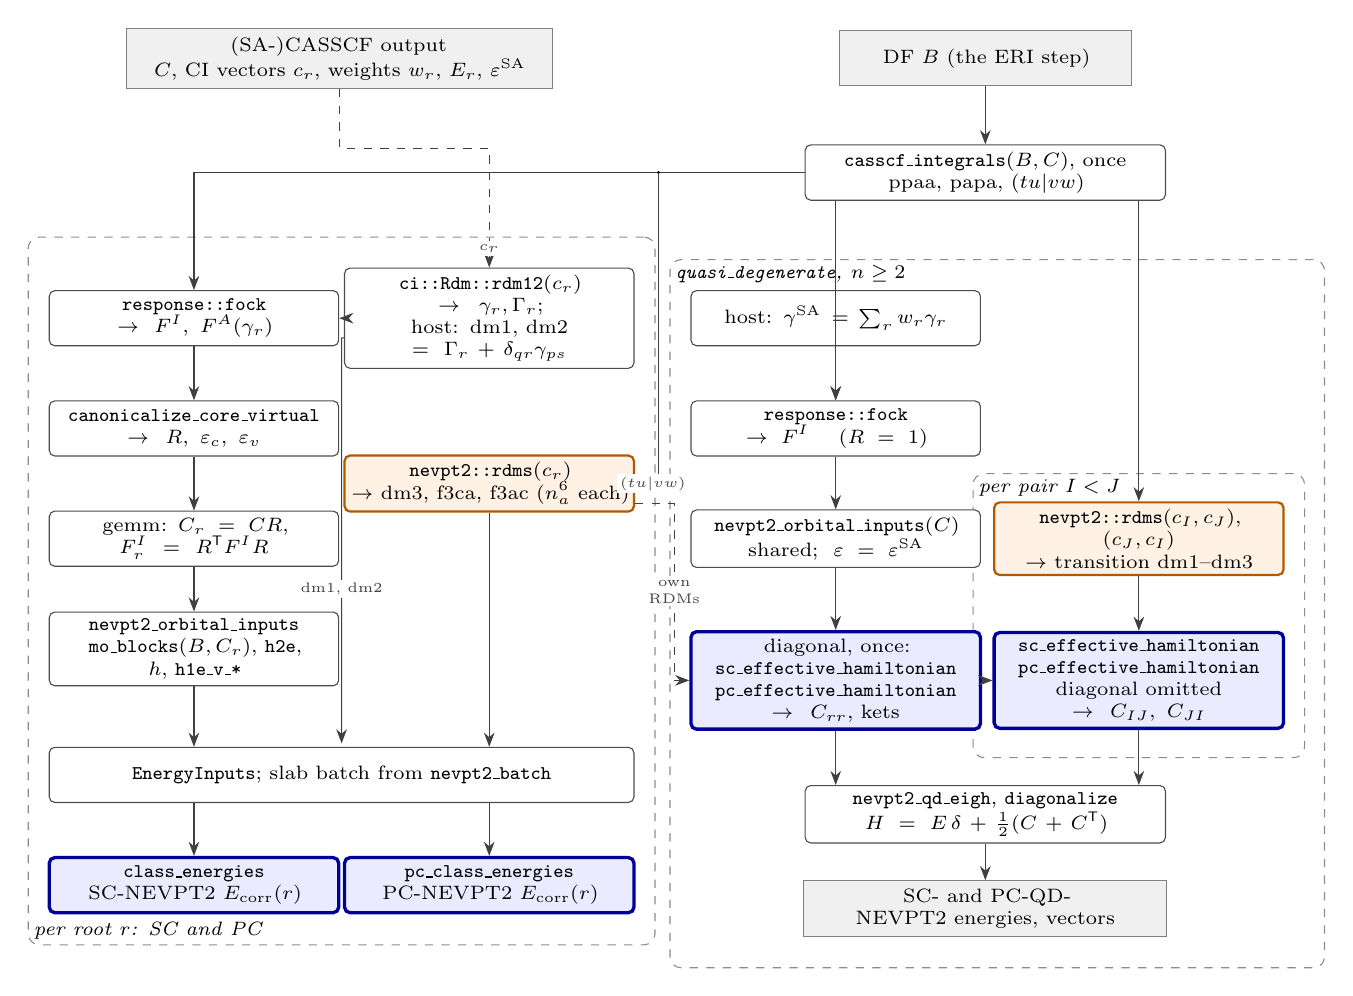
\begin{tikzpicture}[x=1cm, y=1cm]
  \renewcommand{\code}[1]{{\fontsize{7}{8.5}\selectfont\ttfamily #1}}
  \tikzset{fn/.default=3.5cm, entry/.default=3.5cm, hot/.default=3.5cm, data/.default=3.5cm}
  % inputs and shared setup
  \node[data=5.2cm] (cas) at (3.7, 0)
    {(SA-)CASSCF output\\ $C$, CI vectors $c_r$, weights $w_r$, $E_r$, $\eps^{\mathrm{SA}}$};
  \node[data] (b) at (11.9, 0) {DF $B$ (the ERI step)};
  \node[fn=4.4cm] (ints) at (11.9, -1.45)
    {\code{casscf\_integrals}$(B, C)$, once\\ ppaa, papa, $(tu|vw)$};

  % per root: orbital chain (A) and RDM chain (B)
  \node[fn] (fock) at (1.85, -3.3) {\code{response::fock}\\ $\to F^I,\ F^A(\gamma_r)$};
  \node[fn] (canon) at (1.85, -4.7) {\code{canonicalize\_core\_virtual}\\ $\to R,\ \eps_c,\ \eps_v$};
  \node[fn] (rot) at (1.85, -6.1) {gemm: $C_r = CR$,\ \ $F^I_r = R^{\mathsf T}F^I R$};
  \node[fn] (orb) at (1.85, -7.5)
    {\code{nevpt2\_orbital\_inputs}\\ \code{mo\_blocks}$(B, C_r)$, \code{h2e},\\ $h$, \code{h1e\_v\_*}};
  \node[fn] (rdm12) at (5.6, -3.3)
    {\code{ci::Rdm::rdm12}$(c_r)$ $\to\gamma_r,\Gamma_r$;\\ host: dm1, dm2 $=\Gamma_r+\delta_{qr}\gamma_{ps}$};
  \node[hot] (rdms) at (5.6, -5.4) {\code{nevpt2::rdms}$(c_r)$\\ $\to$ dm3, f3ca, f3ac ($n_a^6$ each)};
  \node[fn=7.25cm] (inp) at (3.725, -9.1) {\code{EnergyInputs}; slab batch from \code{nevpt2\_batch}};
  \node[entry] (sc) at (1.85, -10.5) {\code{class\_energies}\\ SC-NEVPT2 $\Ecorr(r)$};
  \node[entry] (pc) at (5.6, -10.5) {\code{pc\_class\_energies}\\ PC-NEVPT2 $\Ecorr(r)$};

  % QD: shared orbitals (C) and pairs (D)
  \node[fn] (gsa) at (10.0, -3.3) {host: $\gamma^{\mathrm{SA}} = \sum_r w_r\gamma_r$};
  \node[fn] (fsa) at (10.0, -4.7) {\code{response::fock}\\ $\to F^I$ \quad($R = 1$)};
  \node[fn] (orbq) at (10.0, -6.1)
    {\code{nevpt2\_orbital\_inputs}$(C)$\\ shared;\ \ $\eps = \eps^{\mathrm{SA}}$};
  \node[entry] (diag) at (10.0, -7.9)
    {diagonal, once:\\ \code{sc\_effective\_hamiltonian}\\ \code{pc\_effective\_hamiltonian}\\ $\to C_{rr}$, kets};
  \node[hot] (trdm) at (13.85, -6.1)
    {\code{nevpt2::rdms}$(c_I, c_J)$, $(c_J, c_I)$\\ $\to$ transition dm1--dm3};
  \node[entry] (pair) at (13.85, -7.9)
    {\code{sc\_effective\_hamiltonian}\\ \code{pc\_effective\_hamiltonian}\\ diagonal omitted\\ $\to C_{IJ},\ C_{JI}$};
  \node[fn=4.4cm] (eigh) at (11.9, -9.6)
    {\code{nevpt2\_qd\_eigh}, \code{diagonalize}\\ $H = E\,\delta + \tfrac12(C + C^{\mathsf T})$};
  \node[data=4.4cm] (qdout) at (11.9, -10.8)
    {SC- and PC-QD-NEVPT2 energies, vectors};

  % groups
  \begin{scope}[on background layer]
    \node[group, fit=(fock)(rdm12)(orb)(inp)(sc)(pc), inner ysep=11pt] (gr) {};
    \node[group, fit=(trdm)(pair), inner ysep=10pt] (gp) {};
    \node[group, fit=(gsa)(fsa)(orbq)(diag)(gp)(eigh)(qdout), inner ysep=11pt] (gq) {};
  \end{scope}
  \node[grouplabel, anchor=south west] at (gr.south west) {per root $r$: SC and PC};
  \node[grouplabel] at (gq.north west) {\code{quasi\_degenerate}, $n \ge 2$};
  \node[grouplabel] at (gp.north west) {per pair $I<J$};

  % the integrals' bus: across to the orbital chain, down the channel
  \draw[arr] (b) -- (ints);
  \draw[arr] (ints.west) -| (fock.north);
  \fill (7.75, -1.45) circle (0.6pt);
  \draw[arr] (7.75, -1.45) |- node[edgelabel, pos=0.62] {$(tu|vw)$} (rdms.east);
  \draw[arr] (ints.south -| fsa) -- (fsa.north);
  \draw[arr] (ints.south -| trdm) -- (trdm.north);
  \draw[side] (cas.south) -- ++(0,-0.75) -| node[edgelabel, pos=0.92] {$c_r$} (rdm12.north);

  % per root
  \draw[arr] (rdm12.west) -- (fock.east);
  \draw[arr] (fock) -- (canon);
  \draw[arr] (canon) -- (rot);
  \draw[arr] (rot) -- (orb);
  \draw[arr] (orb.south) -- (orb.south |- inp.north);
  \draw[arr] ([yshift=-2.5mm]rdm12.west) -- (3.725, -3.55) -- node[edgelabel, pos=0.62] {dm1, dm2} (3.725, -8.7);
  \draw[arr] (rdms.south) -- (rdms.south |- inp.north);
  \draw[arr] (inp.south -| sc) -- (sc.north);
  \draw[arr] (inp.south -| pc) -- (pc.north);

  % QD
  \draw[arr] (gsa) -- (fsa);
  \draw[arr] (fsa) -- (orbq);
  \draw[arr] (orbq) -- (diag);
  \draw[arr] (trdm) -- (pair);
  \draw[arr] (diag) -- (pair);
  \draw[arr] (diag.south) -- (diag.south |- eigh.north);
  \draw[arr] (pair.south) -- (pair.south |- eigh.north);
  \draw[arr] (eigh) -- (qdout);
  \draw[side] ([yshift=-2.5mm]rdms.east) -- (7.95, -5.65) |- node[edgelabel, pos=0.25, align=center]
    {own\\ RDMs} (diag.west);
\end{tikzpicture}
\caption{\code{Nevpt2Step::run} (\code{src/pipeline/nevpt2/nevpt2.cpp}).
Left, every root's own orbitals and RDMs, for SC- and PC-NEVPT2. Right, the
shared state-averaged orbitals for QD: the diagonal is walked once and hands
its first-order wave functions (the kets) and its inputs to the pair calls, which build only
transition RDMs and walk only the transition norms. $C$ and the CI vectors
reach every node that names them; dashed edges carry data from the CASSCF or
across the two passes.}
\label{fig:dag-step}
\end{figure}

\begin{figure}[p]
\centering
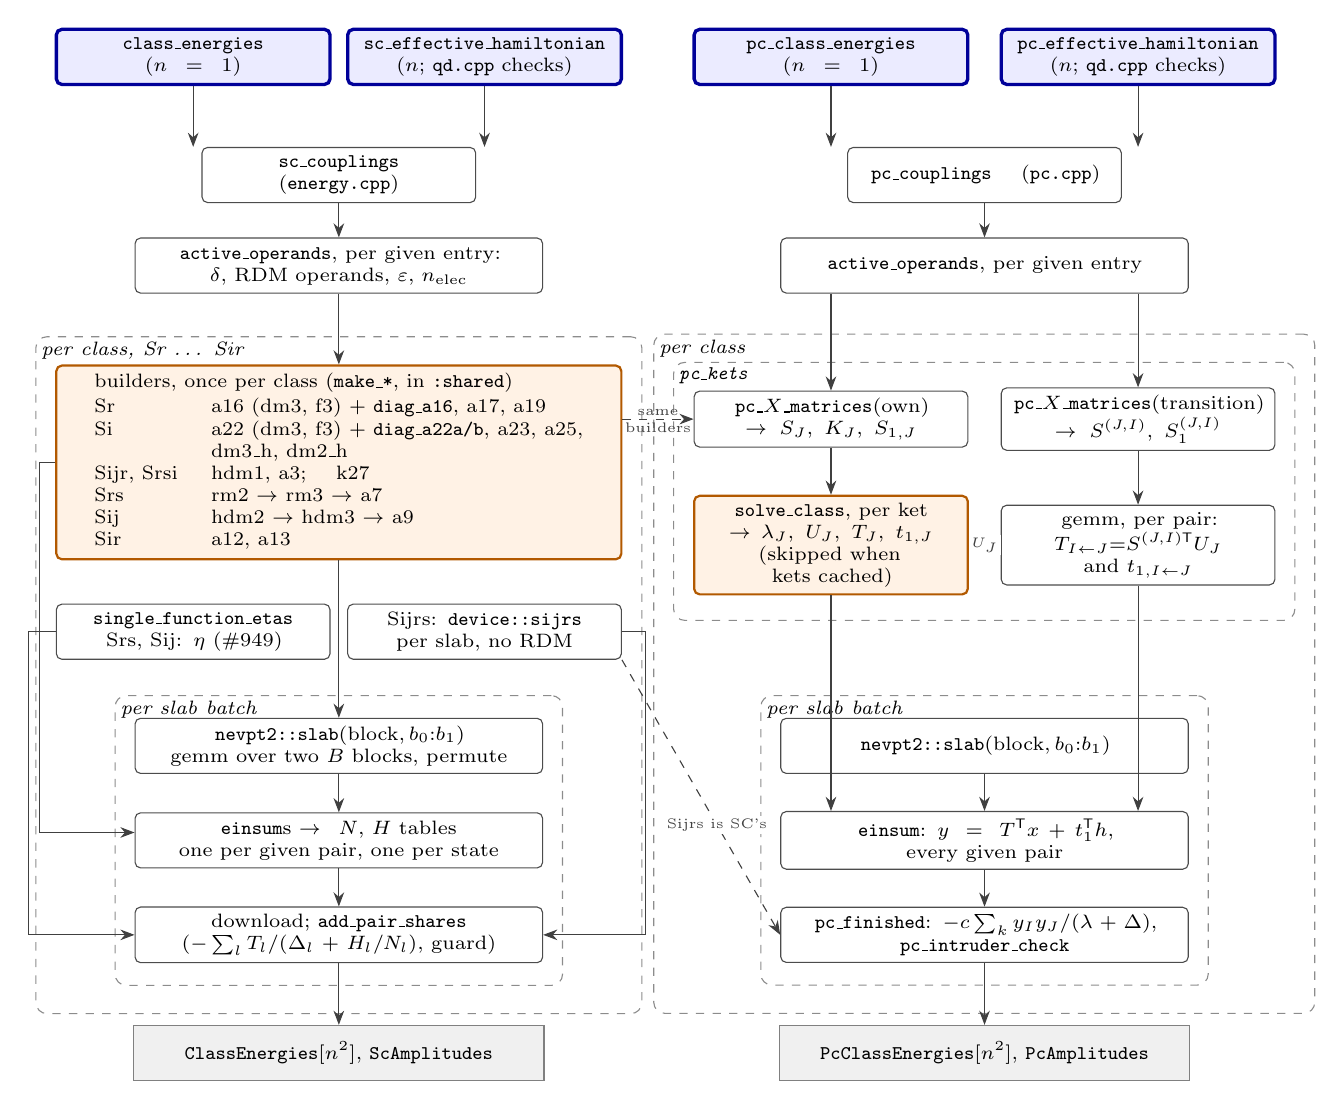
\begin{tikzpicture}[x=1cm, y=1cm]
  \renewcommand{\code}[1]{{\fontsize{7}{8.5}\selectfont\ttfamily #1}}
  % entry points
  \node[entry] (ce) at (1.9, 0) {\code{class\_energies}\\ ($n = 1$)};
  \node[entry] (seh) at (5.6, 0) {\code{sc\_effective\_hamiltonian}\\ ($n$; \code{qd.cpp} checks)};
  \node[entry] (pce) at (10.0, 0) {\code{pc\_class\_energies}\\ ($n = 1$)};
  \node[entry] (peh) at (13.9, 0) {\code{pc\_effective\_hamiltonian}\\ ($n$; \code{qd.cpp} checks)};
  \node[fn] (scc) at (3.75, -1.5) {\code{sc\_couplings} \quad(\code{energy.cpp})};
  \node[fn] (pcc) at (11.95, -1.5) {\code{pc\_couplings} \quad(\code{pc.cpp})};
  \node[fn=5cm] (aos) at (3.75, -2.65)
    {\code{active\_operands}, per given entry:\\ $\delta$, RDM operands, $\eps$, $n_{\mathrm{elec}}$};
  \node[fn=5cm] (aop) at (11.95, -2.65)
    {\code{active\_operands}, per given entry};

  % SC: per class
  \node[hot=7cm] (bld) at (3.75, -5.15) {%
    \begin{tabular}{@{}l l@{}}
    \multicolumn{2}{@{}l}{builders, once per class (\code{make\_*}, in \code{:shared})} \\[1pt]
    Sr  & a16 (dm3, f3) $+$ \code{diag\_a16}, a17, a19 \\
    Si  & a22 (dm3, f3) $+$ \code{diag\_a22a/b}, a23, a25, \\
        & dm3\_h, dm2\_h \\
    Sijr, Srsi & hdm1, a3; \quad k27 \\
    Srs & rm2 $\to$ rm3 $\to$ a7 \\
    Sij & hdm2 $\to$ hdm3 $\to$ a9 \\
    Sir & a12, a13
    \end{tabular}};
  \node[fn] (eta) at (1.9, -7.3) {\code{single\_function\_etas}\\ Srs, Sij: $\eta$ (\#949)};
  \node[fn] (sijrs) at (5.6, -7.3) {Sijrs: \code{device::sijrs}\\ per slab, no RDM};
  \node[fn=5cm] (slab) at (3.75, -8.75) {\code{nevpt2::slab}$(\text{block}, b_0{:}b_1)$\\ gemm over two $B$ blocks, permute};
  \node[fn=5cm] (ein) at (3.75, -9.95) {\code{einsum}s $\to N$, $H$ tables\\ one per given pair, one per state};
  \node[fn=5cm] (fin) at (3.75, -11.15)
    {download; \code{add\_pair\_shares}\\ ($-\sum_l T_l / (\Delta_l + H_l/N_l)$, guard)};
  \node[data=5cm] (outs) at (3.75, -12.65) {\code{ClassEnergies}$[n^2]$, \code{ScAmplitudes}};

  % PC: per class
  \node[fn] (mats) at (10.0, -4.6) {\code{pc\_$X$\_matrices}(own)\\ $\to S_J,\ K_J,\ S_{1,J}$};
  \node[fn] (matt) at (13.9, -4.6) {\code{pc\_$X$\_matrices}(transition)\\ $\to S^{(J,I)},\ S_1^{(J,I)}$};
  \node[hot] (solve) at (10.0, -6.2)
    {\code{solve\_class}, per ket\\ $\to \lambda_J,\ U_J,\ T_J,\ t_{1,J}$\\ (skipped when kets cached)};
  \node[fn] (tg) at (13.9, -6.2) {gemm, per pair:\\ $T_{I\leftarrow J}{=}S^{(J,I)\mathsf T}U_J$\\ and $t_{1,I\leftarrow J}$};
  \node[fn=5cm] (slabp) at (11.95, -8.75) {\code{nevpt2::slab}$(\text{block}, b_0{:}b_1)$};
  \node[fn=5cm] (einp) at (11.95, -9.95) {\code{einsum}: $y = T^{\mathsf T}x + t_1^{\mathsf T}h$,\\ every given pair};
  \node[fn=5cm] (finp) at (11.95, -11.15)
    {\code{pc\_finished}: $-c\sum_k y_I y_J / (\lambda + \Delta)$,\\ \code{pc\_intruder\_check}};
  \node[data=5cm] (outp) at (11.95, -12.65) {\code{PcClassEnergies}$[n^2]$, \code{PcAmplitudes}};

  % groups
  \begin{scope}[on background layer]
    \node[group, fit=(slab)(ein)(fin), inner ysep=8pt] (bs) {};
    \node[group, fit=(bld)(eta)(sijrs)(bs), inner ysep=10pt] (cs) {};
    \node[group, fit=(mats)(matt)(solve)(tg), inner ysep=9pt] (pk) {};
    \node[group, fit=(slabp)(einp)(finp), inner ysep=8pt] (bp) {};
    \node[group, fit=(pk)(bp), inner ysep=10pt] (cp) {};
  \end{scope}
  \node[grouplabel] at (cs.north west) {per class, Sr \ldots\ Sir};
  \node[grouplabel] at (bs.north west) {per slab batch};
  \node[grouplabel] at (cp.north west) {per class};
  \node[grouplabel] at (pk.north west) {\code{pc\_kets}};
  \node[grouplabel] at (bp.north west) {per slab batch};

  % edges: SC
  \draw[arr] (ce.south) -- (ce.south |- scc.north);
  \draw[arr] (seh.south) -- (seh.south |- scc.north);
  \draw[arr] (scc) -- (aos);
  \draw[arr] (aos) -- (bld);
  \draw[arr] (bld.south -| slab.north) ++(0,0) -- (slab.north);
  \draw[arr] (slab) -- (ein);
  \draw[arr] (ein) -- (fin);
  \draw[arr] (fin) -- (outs);
  \draw[arr] (eta.west) -- ++(-0.35,0) |- (fin.west);
  \draw[arr] (sijrs.east) -- ++(0.3,0) |- (fin.east);
  \draw[arr] (bld.west) -- ++(-0.2,0) |- ([yshift=1mm]ein.west);
  % edges: PC
  \draw[arr] (pce.south) -- (pce.south |- pcc.north);
  \draw[arr] (peh.south) -- (peh.south |- pcc.north);
  \draw[arr] (pcc) -- (aop);
  \draw[arr] (aop.south -| mats) -- (mats.north);
  \draw[arr] (aop.south -| matt) -- (matt.north);
  \draw[arr] (mats) -- (solve);
  \draw[arr] (matt) -- (tg);
  \draw[arr] (solve) -- node[edgelabel] {$U_J$} (tg);
  \draw[arr] (solve.south) -- (solve.south |- einp.north);
  \draw[arr] (tg.south) -- (tg.south |- einp.north);
  \draw[arr] (slabp) -- (einp);
  \draw[arr] (einp) -- (finp);
  \draw[arr] (finp) -- (outp);
  % cross edges
  \draw[side] (bld.east |- mats.west) -- node[above, font=\tiny, inner sep=1pt] {same} node[below, font=\tiny, inner sep=1pt] {builders} (mats.west);
  \draw[side] (sijrs.south east) -- node[edgelabel, pos=0.6] {Sijrs is SC's} (finp.west);
\end{tikzpicture}
\caption{Inside \code{free\_breakfast.nevpt2.energy}. Each single-state call
is its effective Hamiltonian's walk at $n = 1$. A class builds its RDM
intermediates once, then walks its external index in batches, building one
slab of the density-fitted integrals at a time. PC solves each ket's metric
once per class (\code{solve\_class}) and reads the slab only through one
einsum into that eigenbasis. With the diagonal omitted, both read the kets
from the amplitudes a diagonal call returned and solve nothing.}
\label{fig:dag-layer}
\end{figure}

%======================================================================
\section{The reverse passes}
\label{sec:reverse}

\subsection{One derivative rule}

\code{einsum\_adjoint} takes a forward einsum's subscripts, operands, output
shape and scale unchanged, and writes operand $k$'s bar as the same einsum
with the output and operand $k$ swapping roles. An operand that repeats a
label takes its bar over its distinct labels and is scattered onto the
diagonal; a strided view takes its bar packed and one GEMM-add places it.
Every class lists its norm and $H$ terms once, as data, and both directions
read the list, so no derivative of a class is transcribed by hand. The
NumPy slice assignments of the reference (\code{a16[:, i, :, :, :, i] += fdm2}
and two in a22) have the gather $\mathrm{fdm2}^\T$-bar $=$
\code{einsum("pirabi->prab", a16\_bar)} as their adjoint, since an input label
may repeat.

\subsection{The SC finish}

The only hand-differentiated expression on the SC side is Eq.~\eqref{eq:sc}'s
finish. With $T_t = -1/(\Delta_t + H_t/N_t)$ \cite{park2019}:
\begin{equation}
  P_t = \frac{\partial E}{\partial N_t} = 2T_t + \Delta_t T_t^2,\qquad
  Q_t = \frac{\partial E}{\partial H_t} = T_t^2,\qquad
  R_t = \frac{\partial E}{\partial \Delta_t} = N_t T_t^2,
  \label{eq:pqr}
\end{equation}
zero for a dropped perturber. A one-function class puts $P_t = c_t$ on
$N_t$, nothing on $H_t$, $\bar D_t = \bar H_{JJ}N_tc_t^2$ (plus the QD share) on
$\Delta_t$, and $\bar\eta = \sum_t\bar D_t$ onto its blocks after the walk:
$\bar\eta\,Y/\langle Y,Y\rangle$ on $X$ and
$\bar\eta\,(X - 2\eta Y)/\langle Y,Y\rangle$ on $Y$. $P$ and $Q$ go back through the norm and $H$
einsums onto the slabs (and so $\Lb$), the one-body rows and the blocks'
bars $M_G = \partial E/\partial G$; $R$ goes onto the orbital energies
$\Delta_t$ reads. Sijrs has its own kernel. Srsi walks twice, since its
finish pairs entries across slabs.

\paragraph{The sweep.} The block bars are swept back through the builders
that formed them, in reverse topological order (an intermediate's bar is
complete before it is swept), onto $\bar h$, the active $\overline{(tu|vw)}$
and $\overline{\mathrm{dm1}}, \ldots, \overline{\mathrm{f3ac}}$. It has two
halves: the Dyall blocks, which read $h$ and $(tu|vw)$ and only a state's
own walk has, and the metrics, which read only RDMs and are all a QD
transition takes. Intermediates are recomputed, never kept.

\paragraph{Identities from the bars.} Each class energy is homogeneous of
degree one in $(N, H)$, so
\begin{equation}
  \sum_t\bigl(P_t N_t + Q_t H_t\bigr) = \sum_G\langle M_G, G\rangle = E_k
  \label{eq:eq40}
\end{equation}
(Park's Eq.~40 \cite{park2019}); and at fixed orbital energies $E$ is
homogeneous of degree 4 in $(B, h_v^{1/2})$, so $\langle\Lb, B\rangle +
2\sum\langle\bar h_v, h_v\rangle = 4E$, $h_v$ the one-body rows. Both are
step-free checks of the bars.

\subsection{The PC solve, backwards}

With $A_t = K + \Delta_t S$ and $x = A_t^{+}b_t$ the solve the energy ran,
\begin{equation}
  \dot E_t = -c\bigl(2\,x^\T\dot b_t - x^\T\dot A_t\,x\bigr),
  \label{eq:pcdot}
\end{equation}
so no eigenvalue or eigenvector derivative appears. This holds where $S$'s
kept rank is locally constant and $K$ annihilates $S$'s dropped modes, which
holds at an eigenstate for its null modes. With real modes dropped at the
cut (\#853) it is validated at PSB3 against re-converged central differences
to $\max(2\times$ the Richardson bar$,\ 3\sigma_E/h_{\min})$, and keeping
those modes does not move it (\code{src/nevpt2/energy/README.md}). In the eigenbasis, with
$g_t = y_t/(\lambda + \Delta_t)$, each tuple gives $\bar y_t = -2c\,g_t$, a
weight $w_t = c\,g_t$ and $\partial E/\partial\Delta_t = c\,g_t\cdot g_t$;
accumulating $M = \sum_t g_t w_t^\T$ and $M_\Delta = \sum_t\Delta_t g_t w_t^\T$
over the walk,
\begin{equation}
  \frac{\partial E}{\partial K} = U M U^\T,\qquad
  \frac{\partial E}{\partial S} = U\bar\Tc^\T + U M_\Delta U^\T,\qquad
  \frac{\partial E}{\partial S_1} = U\bar t_1^\T,
\end{equation}
symmetrised as the solve symmetrised. Those go back through the einsums
that built $S$, $K$, $S_1$ onto SC's block bars, and SC's sweep takes them
unchanged. At fixed slabs and orbital energies a PC class is homogeneous of
degree one in $(S, S_1, K)$, which gives PC's analogue of Eq.~\eqref{eq:eq40}.

\subsection{The QD reverse passes}

Both QD passes differentiate $L = \sum_{MN}\bar H_{MN}H_{MN}$ for a given
$\bar H$; at $n = 1$, $\bar H = 1$ they are the single-state passes einsum
for einsum.

\paragraph{SC-QD.} With $D_N = \Delta + H^N/N^N$, the coupling $-\bar T_{MN}/D_N$
has three bars:
\begin{equation}
  \frac{\partial L}{\partial\bar T_{MN}} = -\frac{\bar H_{MN}}{D_N},\qquad
  A_N = \sum_M\frac{\bar H_{MN}\bar T_{MN}}{D_N^2},\qquad
  \bigl(\bar N^N, \bar H^N, \bar\Delta\bigr) \mathrel{+}=
  \Bigl(-\frac{A_N H^N}{(N^N)^2},\ \frac{A_N}{N^N},\ A_N\Bigr),
\end{equation}
the first split half and half onto the norm einsums of $(M,N)$ and $(N,M)$.
The walk runs in three parts: each state's tables, evaluated only; each
unordered pair, its norm einsums evaluated and differentiated at once, its
metric bars swept onto its transition dm1--dm3 and handed to a callback,
then freed; each state's own walk with $A_N$ added. Memory is one pair's
transition set at a time, never $n^2$ sets.

\paragraph{PC-QD.} The coupling is bilinear in the two rows, so with $g_M =
y_{M\leftarrow N}/(\lambda_N+\Delta)$ and $g = y_N/(\lambda_N+\Delta)$ the
bars are $-c\bar H_{MN}g$ on $y_{M\leftarrow N}$, $-c\bar H_{MN}g_M$ on
$y_N$, $c\bar H_{MN}g_M g^\T$ on $M_N$ (and $\Delta$ times it on $M_{\Delta,N}$),
and $c\bar H_{MN}g_M\cdot g$ on $\Delta$. Still no eigenvector derivative:
$b^{M\leftarrow N}$ lies in $S_N$'s kept range, since a mode annihilating
$|N\rangle$ annihilates $\langle N|S^{(N,M)}$. Then
$\partial L/\partial S^{(N,M)} = \bar\Tc_{M\leftarrow N}U_N^\T$ and
$\partial L/\partial S_1^{(N,M)} = U_N\bar t_{1,M\leftarrow N}^\T$,
unsymmetrised, onto pair $(N,M)$'s transition RDMs. Each class walks its
slabs once with every pair, as the forward does.

%======================================================================
\section{The single-state gradient}
\label{sec:ssgrad}

\subsection{The energy as a function of $(h, B, C, c)$}

\code{sc\_energy} and \code{pc\_energy} rebuild everything the class walk
reads from $(h, B)$ in the MO basis of $C$ and the CI vector $c$:
\begin{equation}
  h1e = F^I_{tu},\quad h1e\_v\_si = F^I_{ti},\quad h1e\_v\_sir = F^I_{ai},\quad
  h1e\_v\_sr = F^I_{at} - \sum_u(au|ut),\quad \eps_x = f_{xx},
\end{equation}
dm3, f3ca, f3ac by \code{rdms}, and dm1, dm2 as dm3's traces
(Eq.~\eqref{eq:traces}). Two choices matter:
\begin{itemize}
\item \textbf{$\eps$ moves with $\gamma$.} It is rebuilt from $(h, B, \gamma)$
  at every point, never an input. Holding it fixed differentiates a
  different functional, and a check whose two sides share the omission
  cannot see it.
\item \textbf{The orbitals are taken as they are.} $\eps$ is $f$'s diagonal;
  off canonical orbitals nothing re-canonicalises. SC-NEVPT2 is not invariant
  to core--core or virtual--virtual rotations, so the pseudocanonical
  conditions $f_{ij} = f_{ab} = 0$ belong to the Lagrangian, not the
  functional.
\end{itemize}
Beyond the five MO blocks the builders read $B_{cc}$ whole and $B_{vv}$'s
diagonal.

\subsection{The adjoints and the orbital source term}
\label{sec:adjoints}

$(h, B)$ in the MO basis is the interface because every NEVPT2 input is
built from it: the orbital energies, the inactive Fock blocks, the active
$(tu|vw)$ and every external slab. So one reverse pass reaches the whole
energy, and both the orbital rotations and the nuclear derivative
integrals act on $(h, B)$ alone. One reverse pass (\S\ref{sec:reverse}, then the builders backwards,
\code{rdms\_adjoint} and the DF adjoints) gives
\begin{equation}
  \hb = \frac{\partial\Ecorr}{\partial h},\qquad
  \Lb^L = \frac{\partial\Ecorr}{\partial B^L},\qquad
  y = \frac{\partial\Ecorr}{\partial c}\Big|_{h,B},
\end{equation}
$\hb$ and each $\Lb^L$ symmetrised last. Along $C \to C(1+\theta)$, any
$\Phi(h, B)$ with symmetric adjoints moves by $\sum\theta_{xy}X_{xy}$,
\begin{equation}
  X = 2\,h\,\hb + 2\sum_L B^L\Lb^L,\qquad
  A = X - X^\T = \frac{\partial\Phi}{\partial\kappa},
  \label{eq:X}
\end{equation}
$X$ needs $B^L_{xq}$ with $x$ general, which is the full-range $B$ or,
without forming it, an AO half-transform:
\begin{equation}
  X = 2\,C^\T h^{\mathrm{AO}}C\,\hb
    + 2\sum_L C^\T J^L\bigl(C\,\Lb^L\bigr),\qquad
  J^L_{\mu\nu} = \sum_P (L^{-1})_{LP}\,(\mu\nu|P),
  \label{eq:Xao}
\end{equation}
evaluated as $\tilde\Lb_q = \Lb_q C^\T$ per $q$ (one batched GEMM), then
$D = B_{\mathrm{AO}}^\T\tilde\Lb$, the DF-exchange shape, rather than pair by
pair. It is exact by construction: $\langle\kappa, A\rangle$ equals the
forward tangent $\dot E(\kappa)$, a check rather than an assembly route. Every block of $A$ has a reader: the mixed blocks
the Z-vector, core--core and virtual--virtual $z^c$, active--active the
gauge identity. $A$ is Park's orbital source term $Y'$ \cite{park2019}.

\subsection{The pseudocanonical multipliers}
\label{sec:zc}

Along $\kappa_{pq} = -\kappa_{qp} = \theta$ within the core or the virtuals,
$f_{pq}$ and $f_{qp}$ move by $\theta(\eps_p - \eps_q)$ and nothing else the
constraint reads moves at first order. So stationarity of $\Ecorr +
\langle z^c, f\rangle$ (full Frobenius sum, symmetric $z^c$) decouples pair
by pair:
\begin{equation}
  z^c_{pq} = z^c_{qp} = -\frac{A_{pq}}{2(\eps_p - \eps_q)},\qquad
  p\ne q\ \text{both core or both virtual},
  \label{eq:zc}
\end{equation}
Park's Eqs.~56--57 \cite{park2019} and Eqs.~25--26 \cite{park2020} in this
tree's sign of $\kappa$. \code{zc\_multipliers} takes only $A$ and $\eps$, so
it serves SC, PC and QD alike.

\paragraph{Degenerate pairs.} For $|\eps_p - \eps_q| < 10^{-6}\,E_h$, a pair
with $|A_{pq}| > 10^{-8}$ is refused, naming both orbitals; one with $A_{pq}$
under its rounding bound ($n_{\mathrm{mo}}^2$ unit roundoffs of $\max|A|$;
partners in different irreps, say) has $z^c_{pq} = 0$; any other keeps
Eq.~\eqref{eq:zc}. PC's $A$ vanishes with the gap,
$A_{pq} = (\eps_p - \eps_q) K_{pq}$ with $K_{pq}$ finite, so PC's $z^c$ has
the limit $-K_{pq}/2$ where SC's grows as the inverse gap and is refused:
this is Park's reason for preferring PC \cite{park2019}. Dropping PC's $z^c$
there would be a step of $O(z)$ in the gradient, not $O(\text{gap})$
(\#974; \code{src/nevpt2/gradient/README.md}, ``Degenerate pairs'').

\paragraph{The term $z^c$ adds.} $\Phi = \langle z^c, f\rangle$ with $D = 2$ on
the core diagonal and $\gamma$ (or $\gamma^{\mathrm{SA}}$) on the active
block, $g_L = \sum B^L_{rs}D_{rs}$ and $w_L = \sum B^L_{pq}z_{pq}$:
\begin{align}
  \Phi &= \langle z, h\rangle + \sum_L w_L g_L - \tfrac12\sum_L\tr(zB^LDB^L),\qquad
  \hb^\Phi = z,\\
  \Lb^{\Phi,L} &= z g_L + D w_L - \tfrac12(zB^LD + DB^Lz),\\
  \mathcal W &= \frac{\partial\Phi}{\partial\gamma} = \sum_L w_L B^L_{aa} - \tfrac12\sum_L(B^LzB^L)_{aa},\\
  y^c_r & = w_r\sum_{tu}(\mathcal W + \mathcal W^\T)_{tu}\,E_{tu}c_r,
\end{align}
the last one sigma-vector application of a one-body operator, batched over
the roots. $y^c$ is raw (not projected), as $y$ is.

\subsection{Lagrangian, Z-vector, gate and nuclear term}

On a converged single-state CASSCF,
\begin{equation}
  \mathcal L = \Ecas + \Ecorr + Z\cdot g_{\mathrm{orb}} + z\cdot g_{\mathrm{ci}} + \langle z^c, f\rangle,
  \qquad g_{\mathrm{ci}} = 2(H_0 - E)c,
  \label{eq:L}
\end{equation}
$g_{\mathrm{orb}}$ \code{response::fock}'s orbital gradient over the packed
non-redundant pairs. Stationarity in the CASSCF parameters
$x = (\kappa_{\mathrm{nr}}, c)$ is the Z-vector equation \cite{handy1984}:
with $J = \partial(g_{\mathrm{orb}}, g_{\mathrm{ci}})/\partial x$, the CASSCF
electronic Hessian, symmetric at a stationary point,
\begin{equation}
  J\begin{pmatrix} Z\\ z\end{pmatrix} = -\begin{pmatrix}
      A^{\mathrm{corr}}_{\mathrm{nr}} + A^{z^c}_{\mathrm{nr}}\\[2pt]
      P_c\bigl(y + y^c\bigr)\end{pmatrix},
  \qquad z\perp c,
  \label{eq:cp}
\end{equation}
$\Ecas$ contributing no right-hand side because $g = 0$. Its blocks are what
the tree has: $J_{\kappa\kappa}$ \code{response::Hessian};
$J_{c\kappa}v = 2P_c(H[v] - \langle H[v]\rangle)c$, $H[v]$ the active
Hamiltonian at the one-index-rotated integrals; $J_{\kappa c}v$ the orbital
gradient at the transition RDMs between $v$ and $c$; and
$J_{cc}v = 2P_c(H - \Ecas)P_cv$, one sigma vector. It is solved by
\code{response::zvector} (preconditioned CG on \code{recipes::pcg}, CI block
projected off $c$ before and after the preconditioner, since $c$ is an exact
null vector of $J_{cc}$): orbital right-hand side
$g + \operatorname{pack}(A^{\mathrm{corr}} + A^{z^c})$ and CI right-hand side
$\tfrac12 P_c(y + y^c)$. The $\tfrac12$ is \code{zvector}'s convention: its
CI row is half of Eq.~\eqref{eq:cp}'s, so a caller of Eq.~\eqref{eq:cp}'s
form scales its CI right-hand side to match.

\paragraph{The total adjoint.} Every term of Eq.~\eqref{eq:L} but $V_{nn}$ is
a function of $(h, B)$ at fixed $(c, Z, z, z^c)$, so the nuclear term reads
the sum of their adjoints,
\begin{equation}
  \hb^{\mathcal L} = \hb^{\mathrm{cas}} + \hb^{\mathrm{corr}} + \hb^{Z} + \hb^{z} + \hb^{z^c},\qquad
  \Lb^{\mathcal L} = \Lb^{\mathrm{cas}} + \Lb^{\mathrm{corr}} + \Lb^{Z} + \Lb^{z} + \Lb^{z^c}:
  \label{eq:total}
\end{equation}
CAS, $\hb^{\mathrm{cas}} = D$ and $\Lb^{\mathrm{cas},L}_{pq} =
\sum_{rs}\Gamma_{pqrs}B^L_{rs}$ (the core parts J/K shapes, the active part
$\G2$ against $B_{aa}$); $Z$, $\Ecas$'s adjoints at the rotated densities
$D^Z = Z^\T D + DZ$ and their four-index analogue; $z$, $\Ecas$'s at the
symmetrised transition densities between $z$ and $c$, times 2; $z^c$, $\Phi$'s
above; corr, the reverse pass.

\paragraph{The gate: a free, exact check of the whole solve.} $\mathcal L$
is stationary in every rotation, so by Eq.~\eqref{eq:X} its total
$X^{\mathcal L}$ must be symmetric in every block, gauge blocks included. Its antisymmetric part,
\begin{equation}
  A^{\mathcal L} = 2(F - F^\T)\bigl(\gamma + \gamma_z, \Gamma + \Gamma_z\bigr) + A^Z + A^{\mathrm{corr}} + A^{z^c},
\end{equation}
with $F$ the generalised Fock at the root's RDMs plus $z$'s transition RDMs,
and $A^Z = 2(F' - F'^\T)$, $F'$ the derivative of $F$ along $C(1 + \epsilon\kappa(Z))$,
is evaluated and every block past $10^{-8}$ is refused, naming it. $F$ is a
polynomial of degree 4 in $C$, so a five-point stencil gives $F'$ exactly to
round-off. On the non-redundant pairs $A^{\mathcal L}$ is the Z-vector's
residual, on the inactive pairs Eq.~\eqref{eq:zc}'s, on the active pairs the
gauge identity's: a wrong factor in any term names its block.

\paragraph{The nuclear term.} Along any orthonormality-preserving path the
symmetric part of $\theta$ is $-\tfrac12 C^\T S^A C$, so with the total
adjoints $(\hb^{\mathcal L}, \Lb^{\mathcal L}, X^{\mathcal L})$,
\begin{equation}
  \frac{dE}{dR_A} = \sum_{\mu\nu}\mathcal P_{\mu\nu}h^{A}_{\mu\nu}
  + \sum_{\mu\nu P}\mathcal G^P_{\mu\nu}(\mu\nu|P)^{A}
  - \tfrac12\sum_{PQ}\mathcal V_{PQ}(P|Q)^{A}
  - \sum_{\mu\nu}\mathcal W_{\mu\nu}S^{A}_{\mu\nu} + V_{nn}^{A},
  \label{eq:grad}
\end{equation}
$\mathcal P = C\hb^{\mathcal L}C^\T$,
$\mathcal G^P = \sum_L(L^{-\T})_{PL}C\Lb^{\mathcal L,L}C^\T$,
$\mathcal V = L^{-\T}\mathcal G^{\mathrm{aux}}L^{-1}$ with
$\mathcal G^{\mathrm{aux}}_{LL'} = \langle\Lb^{\mathcal L,L}, B^{L'}\rangle$,
and $\mathcal W = \tfrac12 C\,\sym(X^{\mathcal L})C^\T$. In the code this is
one \code{mcscf::df\_gradient} pass: $\Ecas$'s and the multipliers' terms are
the ones it builds, and $(\hb, \Lb, X)$ of $\Ecorr + \Phi$ are its
``extra'' MO adjoint. No relaxed density is formed separately.

\begin{algorithm}[htbp]
\caption{The DF-NEVPT2 nuclear gradient (\code{sc\_gradient}, \code{pc\_gradient})}
\label{alg:ssgrad}
\begin{algorithmic}[1]
\Require converged single-state DF-CASSCF $(C, c)$, core and virtuals canonical; SC or PC
\Ensure $dE/dR$
\State $(\Ecorr, \hb, \Lb, y, X, A, \eps) \gets$ \code{sc\_adjoint} or \code{pc\_adjoint}
\State $z^c \gets$ Eq.~\eqref{eq:zc}; refuse an undetermined degenerate pair
\State $(\Phi, \hb^\Phi, \Lb^\Phi, y^c, X^\Phi, A^\Phi) \gets$ \code{zc\_adjoint}; add field by field
\State $(Z, z) \gets$ \code{zvector}$\bigl(g + \operatorname{pack}A,\ \tfrac12(y + y^c)\bigr)$
\State \textbf{gate:} $A^{\mathcal L}$ below $10^{-8}$ in all six blocks
\State $dE/dR \gets$ \code{df\_gradient}$\bigl(\text{multipliers } (Z,z),\ \text{extra } (\hb, \Lb, X)\bigr)$
\end{algorithmic}
\end{algorithm}

%======================================================================
\section{The single-state nuclear Hessian}
\label{sec:hessian}

\code{hessian::df\_sc\_nevpt2} and \code{hessian::df\_pc\_nevpt2} (\#816,
\#817) return $d^2(\Ecas + \Ecorr)/dR_A\,dR_B$ on a converged single-state
DF-CASSCF, in $k$ coordinates $q_i = \sum_x Q_{ix}R_x$ (orthonormal rows, the
Cartesian ones when none are given). They are all-electron, and a state
average or a frozen core is refused. They are assembled in \code{hessian}
from this layer's tangents and Hessian-vector products and from the CASSCF
Hessian's parts, with no integrals of their own. There is no QD-NEVPT2
Hessian.

\subsection{The $2n+1$ form}

Collect the pieces of Eq.~\eqref{eq:L}: the parameters
$x = (\kappa_{\mathrm{nr}}, \kappa_{oo}, c)$, the non-redundant CASSCF
rotations, the core--core and virtual--virtual rotations the
pseudocanonical condition pins, and the CI vector; the multipliers
$\lambda = (Z, z, z^c)$; the constraints
$g = (g_{\mathrm{orb}}, g_{\mathrm{ci}}, f_{oo})$. At the solution
$\Lag_x = 0$ and $g = 0$, so $dE/dR_A = \Lag_A$ at fixed $(x, \lambda)$
along an orthonormal path. Differentiating once more and eliminating
$\lambda_B$ with the two first-order conditions, $g_A + g_x x_A = 0$ and
$\Lag_{xB} + \Lag_{xx}x_B + g_x^\T\lambda_B = 0$,
\begin{equation}
  \frac{d^2E}{dR_A\,dR_B} = \Lag_{AB} + \Lag_{Ax}\,x_B + x_A^\T\Lag_{xB}
    + x_A^\T\,\Lag_{xx}\,x_B,
  \qquad g_x\,x_A = -g_A.
  \label{eq:hess}
\end{equation}
The parameters are needed to first order, one linear solve per coordinate.
The multipliers are the gradient's own, at zeroth order, so their $3N$
responses never appear, and no second-order response $x_{AB}$ does either.
SC's amplitudes are closed form and PC's come from a solve whose
factorisation the tangent reuses, so neither needs an amplitude response of
its own.

\subsection{The parameter response and the tangent}

$g_x$ is block triangular: the CASSCF constraints transform covariantly
under $\kappa_{oo}$ and do not respond to it at a stationary point.
\begin{enumerate}
\item \textbf{CP-CASSCF}, $J(\kappa_{\mathrm{nr}}, c)_A = -\partial
  g_{\mathrm{CAS}}/\partial R_A$, $J$ the gradient's CI-relaxed Hessian:
  \code{hessian::df\_casscf}'s step (or \code{df\_casscf\_cp} alone),
  \code{response::zvectors} on all $3N$ columns at once, CI right-hand sides
  halved to the Z-vector's convention. A state-specific excited root is a
  saddle in $(\kappa, c)$ and is refused (Divergence); so is a singular
  $\tilde H$, detected by a probe column (\#978).
\item \textbf{The pseudocanonical block}, closed form once 1.\ is done:
  \begin{equation}
    \kappa^A_{pq} = -\frac{f^{(A)}_{pq}}{\eps_p - \eps_q},\qquad
    (p, q)\ \text{core--core or virtual--virtual},
    \label{eq:koo}
  \end{equation}
  $f^{(A)}$ the total first-order change of $f$ at fixed $\kappa_{oo}$.
  Below $|\eps_p - \eps_q| = 10^{-6}$, $\kappa^A_{pq} = 0$ while
  $|f^{(A)}_{pq}| \le 10^{-8}$ (a split the displacement does not lift);
  past that SC refuses, naming the pair and the coordinate, and PC records a
  degenerate pair, which its Hessian refuses (\S\ref{sec:hess-refusals}).
\end{enumerate}
Eq.~\eqref{eq:koo} is $z^c$'s division again, now in a response that
enters Eq.~\eqref{eq:hess} quadratically. PC does not escape it: this tree's
PC puts each tuple at its own $\Delta_t$ from $f$'s diagonal and is not
invariant to inactive rotations, so $\kappa_{oo}$ stays in PC's Hessian too.

\code{hessian::df\_nevpt2\_tangents} then forms the total first-order change
of the NEVPT2 functional's inputs along each coordinate, in the MO basis:
\begin{equation}
  \dot h^x = h^x + \kappa^{x\T}h + h\kappa^x,\qquad
  \dot B^x_Q = W^x_Q + \kappa^{x\T}B_Q + B_Q\kappa^x,\qquad
  \dot c^x = c^x,\qquad
  \kappa^x = \kappa^x_{\mathrm{nr}} + \kappa^x_{oo},
  \label{eq:tx}
\end{equation}
$(h^x, W^x)$ the derivative integrals along the L\"owdin connection
$\tau^x = -\tfrac12 S^x_{\mathrm{MO}}$ (\code{mcscf::df\_integral\_derivatives}),
$W^x$'s fitted index carried in the gauge $\mu^x = -\tfrac12 m^x$,
$m^x = L^{-1}M^xL^{-\T}$. $f^{(x)}$ comes from \code{nevpt2::builders\_tangent},
the forward tangent of every builder the energy reads, each term by its
product rule over the forward's own builds. The RDMs' tangent is exact in
three \code{rdms} calls: the bra/ket builds at $(\dot c, c)$ and $(c, \dot c)$,
and the one-vector build over $(tu|vw)$'s tangent, of which only f3 is kept.

\subsection{The Hessian-vector product}
\label{sec:hvp}

\code{sc\_hessian\_product} and \code{pc\_hessian\_product} (\#814, \#815)
are the tangent of \code{*\_adjoint} $+$ \code{zc\_adjoint} at fixed $z^c$
along directions $(\dot h, \dot B, \dot c)$, so $\langle t_A,
\mathrm{HVP}\,t_B\rangle$ is the $\Ecorr + \Phi$ share of
Eq.~\eqref{eq:hess} along Eq.~\eqref{eq:tx}'s $t$. The adjoint is $J^\T\bar E$, $\bar E$
the class walk's bars at the builders' outputs and $J$ the builders'
Jacobian, so its tangent is forward over reverse, two kinds of term, one
sweep (\code{bars\_tangent}):
\begin{itemize}
\item $J^\T\dot{\bar E}$: the class walk's bars along the builders' tangent
  (\code{class\_energies\_hvp}, \code{pc\_class\_energies\_hvp}), run back
  through the gradient's own reverse pass;
\item $\dot J^\T\bar E$: every builder term's adjoint at the fixed bars with
  one other operand at its tangent, the same einsum with the operand swapped
  (\code{adjoint\_slot}), so no derivative is written by hand.
\end{itemize}

\paragraph{SC's class tangent.} The multipliers' tangent is the finish's
$3\times3$ Hessian. In the $(N, d)$ form, $d = N\Delta + H$ and $E = -N^2/d$,
which carries no removable $1/N$:
\begin{equation}
\begin{aligned}
  E_{NN} &= -\frac2d + \frac{4N\Delta}{d^2} - \frac{2N^2\Delta^2}{d^3}, &
  E_{NH} &= \frac{2N}{d^2} - \frac{2N^2\Delta}{d^3}, &
  E_{N\Delta} &= \frac{3N^2}{d^2} - \frac{2N^3\Delta}{d^3},\\
  E_{HH} &= -\frac{2N^2}{d^3}, &
  E_{H\Delta} &= -\frac{2N^3}{d^3}, &
  E_{\Delta\Delta} &= -\frac{2N^4}{d^3},
\end{aligned}
\label{eq:finish}
\end{equation}
whose $(H, \Delta)$ block has rank one, and whose degree-one homogeneity in
$(N, H)$ gives $NE_{NN} + HE_{NH} = 0 = NE_{NH} + HE_{HH}$. Times the forward
tangent's $(\dot N, \dot H, \dot\Delta)$ it gives $(\dot P, \dot Q, \dot R)$,
taken onto every bar by one reverse pass at fixed multipliers. The bars at
fixed multipliers are themselves polynomials of degree at most five along a
line (two slabs, each quadratic in $B$, around a block of degree at most
two), so
\begin{equation}
  \sum_{k=1}^{3} w_k\,\frac{A(x + ks\dot x) - A(x - ks\dot x)}{2ks},\qquad
  w = \bigl(\tfrac32, -\tfrac35, \tfrac1{10}\bigr),
\end{equation}
is their derivative exactly, the weights cancelling the $s^2$ and $s^4$
terms. A one-function class reads $\dot\eta$ from the blocks' polarisation.

\paragraph{PC's class tangent.} The same split over the solve. With
$g = y/(\lambda + \Delta)$ the multipliers move as
$\dot g = (\dot y - \dot D g)/(\lambda + \Delta)$,
$\dot D = \dot K' + \Delta\dot S' + \dot\Delta$, the solve differentiated
through its own factorisation. $U$'s tangent $V_n\Theta'$ enters through a
symmetric difference that is exact (the bars are quadratic in $U$), the
inputs' tangent at fixed multipliers through the same three-point formula,
and the kept span's rotation through the Daleckii--Krein derivative of the
span bar. Every divided difference there is a product of two first-order
ones, so no pair on one side of the cut is ever divided by. These are the
null-space rotation terms of $S^+ = UU^\T$: zero for exact null modes at an
eigenstate, and of the first-order term's size for real modes near the cut.

\paragraph{$\Phi$, and the functional of $c$.} $\Phi = \langle z^c,
f\rangle$ is linear in $h$, bilinear in $B$ and quadratic in $c$, so its
share at fixed $z^c$ is closed form. Two conventions fix the CI--CI block,
and the gradient shares both. The product is the Hessian of the
\emph{Rayleigh-normalised} functional $F(h, B, c) = (\Ecorr + \Phi)(h, B,
c/|c|)$, so the sphere's $-(u\cdot v)\,(\partial\Lag/\partial c)\cdot c$ is
included: with $P = 1 - cc^\T$ and $u = \dot c - (c\cdot\dot c)c$, the
c-gradient's tangent is
$P\dot y(\dot h, \dot B, u) - u\,(c\cdot y) - c\,(u\cdot y) - (c\cdot\dot c)Py$.
The off-shell extension is the rank-reduced one, $\hat H_D|\Psi_0\rangle =
E_0|\Psi_0\rangle$ off the root too, with no Kollmar residual
\cite{kollmar2021}. A residual-including CI--CI block against this
gradient's $z$, or the reverse, would be wrong with no symptom.

\subsection{Assembly}
\label{sec:hess-assembly}

Every part is the second derivative of its term of $\Lag$ along one path:
the orbitals $C(R)\exp K$ along the L\"owdin connection
$C(R) = C(C^\T S(R)C)^{-1/2}$, $K = \kappa_{\mathrm{nr}} + \kappa_{oo}$, the CI
vector $\exp(A)c$ on the unit sphere, and $B$'s fitted index in one gauge.
A part in another parametrization would leave a term of second order in
$\kappa$ unaccounted. With $N = \Ecorr + \Phi$ a function of
$I = (h, B)$ and $c$, $O(M, \kappa) = \kappa^\T M + M\kappa$ and
$t_A = I^A + O(I, \kappa^A) + c^A$:
\begin{equation}
\begin{aligned}
  N^{\mathrm{total}}_{AB} &= \langle N_I, I^{AB}\rangle
  + \langle t_A, N''\,t_B\rangle\\
  &\quad + \langle N_I, O(I^A, \kappa^B) + O(I^B, \kappa^A)\rangle
  + \langle N_I, \tfrac12 O(O(I, \kappa^A), \kappa^B) + (A\leftrightarrow B)\rangle,
\end{aligned}
  \label{eq:Nab}
\end{equation}
the skeleton, the product, and the rotation cross terms $\tau\kappa$ and
$\kappa\kappa$. For symmetric $M$, $\langle N_I, O(M, \kappa)\rangle =
\langle\kappa, X(M)\rangle$, $X(M) = 2(M_h\hb + \sum_Q M_Q\Lb_Q)$, so the
cross terms are $n_{\mathrm{mo}}^2$ Gram matrices. The parts and what
computes each:

\begin{center}
\small
\begin{tabularx}{\linewidth}{@{}lX@{}}
\toprule
part & computed by \\
\midrule
$\Ecas$ & \code{hessian::df\_casscf} as is; its $\kappa_{oo}$ rows vanish by $\Ecas(CU, c) = \Ecas(C, c)$ \\
$t_x$ & \code{df\_nevpt2\_tangents} over its $\lambda^x$, with $\kappa^x_{oo}$ \\
$(\hb, \Lb)$, multipliers & \code{*\_adjoint}, \code{zc\_multipliers}, \code{zc\_adjoint}, \code{lagrangian\_gradient}: the gradient's chain, adjoint kept \\
$\langle t_A, N'' t_B\rangle$ & \code{*\_hessian\_product} along each coordinate's $t$, paired with every $t_A$ by three GEMVs \\
$Z$ terms & \code{df\_casscf\_z}: $Z\cdot\partial^2g/\partial R\,\partial R$, $I^xZ$ against $\lambda^y$ both ways, and $\lambda^\T(Z\cdot\partial^2 g)\lambda$, the CASSCF third derivative \\
skeleton & \code{df\_adjoint\_xy}: $\sum\hb\,h^{xy} + \sum\Lb\,B^{xy}$ \\
$\tau\kappa$, $\kappa\kappa$ & $X$ Gram matrices from $n_{\mathrm{mo}}^2$ stacks \\
$\kappa_{oo}$ rows & $\tfrac12\bigl(\langle\kappa^B_{oo}, [X_N, \kappa^A_{\mathrm{nr}}]\rangle + (A\leftrightarrow B)\bigr)$ \\
\bottomrule
\end{tabularx}
\end{center}

\paragraph{The $\kappa_{oo}$ rows} follow from BCH to second order,
$\exp(sP + tQ) = \exp(sP)\exp(tQ)\exp(-\tfrac12 st[P, Q]) + O(3)$, and the
covariance of the orbital gradient: of $Z\cdot g$'s second derivative only
$-\tfrac12\nabla(Z\cdot g)\cdot([\kappa^A_{\mathrm{nr}}, \kappa^B_{oo}] +
[\kappa^B_{\mathrm{nr}}, \kappa^A_{oo}])$ survives, and the Z-vector equation
turns $\nabla(Z\cdot g)$ into $-X_N$. $N$'s own $\kappa_{oo}$ terms are in
$t$'s $\kappa$, so the product and the cross terms carry them.

\paragraph{The skeleton's gauge.} $h_{\mathrm{MO}}$ and $B_{\mathrm{MO}}$ are
differentiated along
$\tau^{xy} = -\tfrac12 S^{xy} + \tfrac38\{S^x, S^y\}$ and, on the fitted
index, $\mu^{xy} = -\tfrac12 m^{xy} + \tfrac38\{m^x, m^y\}$: the symmetric
square root's second order, whose first order is exactly $W^x$'s gauge. The
fitted index is defined only up to an orthogonal turn, which a general
$\Lb$ sees; the product's term pairs $W^x$ and this one $B^{xy}$, and their
sum is the derivative of one function only because both are the same curve.

The result is exactly symmetric; the antisymmetric part discarded and the
translational sum are returned.

\subsection{Where there is no Hessian: the refusals}
\label{sec:hess-refusals}

Each refusal below is Numerical, names what failed, and returns no
Hessian; the CP solve's own (a saddle, a singular $\tilde H$) are passed on
as they come.

\paragraph{SC: empty perturbers.} At a symmetric geometry a perturber can be
empty by symmetry ($|N| \le 10^{-14}$); a direction that breaks the symmetry
populates it at second order, where its energy is homogeneous of degree two
in the direction. Along one direction $u$ it is a quadratic form, and the
perturber takes the demo's K6, the finish's multipliers at the ray's limit
$\eta = H^{uu}/N^{uu}$. Along a pair $(u, v)$ that both populate it, it
takes K6 at the mean $\eta$ and is scored by
$\rho_\tau = \max(|\eta_u - \eta_v|, 2|\kappa - c\eta|)/|\Delta + \eta|$ at
unit populations, zero exactly when $H \propto N$ on the pair, weighted by
the perturber's share of the pair's Hessian (\#914). Past $10^{-6}$ the pair
is refused: the energy is a second derivative along every line but no
bilinear form, \#894's SC kink. Because the product is not linear in the
direction there, the Hessian is taken along each coordinate's own $t$ and
pairs of symmetry-breaking coordinates are taken again as each other's
partners. A coordinate breaks the symmetry when its population exceeds
$10^{-10}$ (\code{kEmptyPopulationFloor}) of the \emph{largest} scale over the
coordinates (\#952: a rigid translation's tangent is round-off and populates
everything against its own scale). At \code{nh3\_cs\_sto3g} in symmetry-adapted
coordinates the whole A$''\times$A$''$ off-diagonal block is refused, which is
the right output.

\paragraph{SC: mixing inactive pairs (\#952).} SC is not invariant to
inactive rotations. Where a coordinate couples two near-degenerate inactive
orbitals, the pair's $2\times2$ block $[[\eps_p, Ft], [Ft, \eps_q]]$ has
gap $\sqrt{g^2 + 4F^2t^2}$, and its avoided crossing has half-width
$t_{\mathrm{mix}} = g/2|F| = 1/(2|\kappa^i_{oo,pq}|)$. Past it the pair has
rotated and the curvature is a different branch's. At \code{examples/nevpt2.toml}'s
C$_{2v}$ water, virtuals 1.4\,m$E_h$ apart give $t_{\mathrm{mix}} =
5.6\times10^{-4}$\,bohr along B$_2$, and SC's B$_2$ frequency is 14063
against PC's 4028\,cm$^{-1}$. The analytic element is the correct $t\to0$
limit, which a ladder of the gradient reaches only below $10^{-4}$\,bohr.
Any coordinate with $t_{\mathrm{mix}} < 10^{-3}$\,bohr is refused, naming the
pair and recommending PC.

\paragraph{PC: no partners, but the Schur lift.} PC has no empty perturbers:
a tuple that vanishes by symmetry has $b = Sx = 0$ and moves as a smooth
quadratic. Instead a null mode $v$ of $S$ can rise at second order along
the CI vector's path. With $S(t) = S + tS' + \tfrac12t^2S''$ the null block's
eigenvalues rise as $\tfrac12t^2\,\mathrm{eig}(L)$,
\begin{equation}
  L = \mathcal P\,(S'' - 2S'S^+S')\,\mathcal P,
\end{equation}
$\mathcal P$ the null projector, $L \succeq 0$. Structural null modes never
lift ($L = 0$), spin ones not along singlet directions, and symmetry ones
do along a singlet that breaks the symmetry. A lifted mode crosses the cut
at $t^* = \sqrt{2\,\mathrm{cut}\,\sigma_{\max}/\ell}$, $\ell = \mathrm{eig}(L)$,
beyond which the energy carries its share. The product stays the exact
derivative of the dropped branch and reports $t^*$ per direction and class.
Along the coordinate's own $t$ (its CI part $c^B$) $t^*$ is in bohr, and any
coordinate and class with $t^* < 10^{-3}$\,bohr is refused. HCN's CAS(6,6)
with its $\sigma$ pair active lifts Sir's modes at $2$--$5\times10^{-4}$\,bohr
on every bend; at $f = 10^{-10}$, $t^*$ grows to $5\times10^{-3}$--$10^{-2}$
and nothing is refused.

\paragraph{PC: thin kept spectra and degenerate pairs.} A class whose
\code{kept} is below $10^{-10}$ of its $\sigma_{\max}$ is refused, naming
the floor that would cut it (\#917; \#943 reaches it at a C$_{2v}$
formaldehyde CAS(6,6)). A degenerate inactive pair that a coordinate splits
(gap below $10^{-6}\,E_h$, $|f^{(x)}_{pq}| > 10^{-8}$) is refused, since
$\kappa^x_{oo}$ is not a division the state determines there. The check is
conservative: any Cartesian record refuses, even if the caller's coordinates
combine them so that $f$ vanishes.

\paragraph{PC near a degenerate pair, measured.} \code{h2co\_neardeg\_sto3g}'s
virtual pair is $6\times10^{-3}\,E_h$ apart, $\max|\kappa^x_{oo}| = 21.8$, and
its reference ladder runs through gaps of $5.6\times10^{-5}$. The terms that
grow as $1/\mathrm{gap}^2$, $\kappa\kappa$ and the product's
$\kappa_{oo}$--$\kappa_{oo}$ block, are each about $10^9$ bars and cancel to
the fixture's bar: about nine of the parts' sixteen digits go into it. So
PC's second-order $\kappa_{oo}$ terms do cancel the $1/(\eps_p - \eps_q)$ of
Eq.~\eqref{eq:koo}, at the cost of digits, and that pair is not refused.

\subsection{The semi-numerical Hessian and the bilinearity check}
\label{sec:seminumerical}

The numerical alternative differences the analytic gradient,
\begin{equation}
  H_{AB} \approx \frac{g_A(R + s\,q_B) - g_A(R - s\,q_B)}{2s},\qquad
  H \leftarrow \tfrac12(H + H^\T),
  \label{eq:semi}
\end{equation}
along each coordinate $q_B$, in the pipeline by a fourth-order stencil.
Each displaced CASSCF starts from the reference's orbitals orthonormalised
in the displaced metric, $C(S_{\mathrm{MO}})^{-1/2}$, and its CI, and passes
the CASSCF chain's continuity guards. It is also the oracle for the analytic
Hessian. It does not escape the differentiability problem of
\S\ref{sec:hess-refusals}: along a pair of directions that leave the
symmetry, a difference converges, if at all, to a polarisation of
directional second derivatives that depends on the step and on the
combination of coordinates.

\paragraph{The diagnostic.} For coordinates $q_1$, $q_2$, check
\begin{equation}
  H(q_1 + q_2,\ q_1 + q_2) \stackrel{?}{=} H(q_1, q_1) + H(q_2, q_2) + 2H(q_1, q_2),
  \label{eq:bilinear}
\end{equation}
with the step dependence of each element. A violation above the difference
noise means that block has no Hessian, and it is reported rather than
published as a frequency. With one coordinate in an irrep
Eq.~\eqref{eq:bilinear} is empty and the ladder is the only evidence.

\paragraph{Which coordinates.} Across two irreps the cross block vanishes
by symmetry in symmetry-adapted coordinates, but the function need not be a
quadratic form there either. A Cartesian step mixes irreps, so a Cartesian
difference Hessian at a symmetric point depends on the frame, silently.
Symmetry-adapted coordinates avoid that and name the failing block; on
Cartesian pairs the check still detects a failure, at two more gradients
per pair, without naming the irrep. The tree detects no point group, so the
coordinates are the caller's (\code{[hessian] coordinates}, orthonormal
rows). Element $(i, j)$ is $q_i^\T\,\partial g/\partial q_j$, and a Cartesian
Hessian is $Q^\T HQ$.

\paragraph{In the pipeline (\#812).} Under \code{[nevpt2\_gradient]} the
numerical \code{[hessian]} runs a ladder by default: each column at $s = h$,
$h/2$, $h/4$, the ratio of successive changes judged in $(12.8, 19.2)$ where
the finer change is past ten noise floors, the floor measured from restarts
and from re-solves at tolerances a hundred times tighter. It checks
Eq.~\eqref{eq:bilinear} on every coordinate pair up to twelve coordinates.
A failing pair withholds the frequencies: the run fails, naming the pairs.
At \code{nh3\_cs\_sto3g} under SC in symmetry-adapted coordinates all ten
A$''\times$A$''$ pairs fail and the cross-irrep pairs pass, which is the
block the analytic route refuses.

\subsection{In the pipeline}

\code{[hessian]} beside a single-state \code{[nevpt2\_gradient]} is that
variant's $\Ecas + \Ecorr$ Hessian (\#818): analytic by default, or
central differences of \code{sc\_gradient}/\code{pc\_gradient} over $6N$
displaced geometries under a Richardson ladder with a bilinearity check
(\#812). \code{coordinates}, when given, are passed through and the result
reported in Cartesians, $Q^\T HQ$: at a symmetric geometry give the
symmetry-adapted ones. Under \code{variant = "pc"} the whole chain runs at
\code{pc\_floor} $= 10^{-10}$ (\code{HessianStep::kPcFloor}), the outer
\code{[nevpt2\_gradient]} included, so the gradient written beside the
Hessian is the same energy's; \code{pc\_floor = 0} restores the round-off
cut bitwise. Refused before anything runs: integral-direct ERIs, a state
average, \code{quasi\_degenerate}, a frozen core and a
\code{[casscf\_gradient]} beside it. Stationarity is assumed, not checked:
converge \code{[casscf]} to \code{conv\_tol\_grad} $= 10^{-10}$. Harmonic
analysis follows; there are no IR intensities.

%======================================================================
\section{The QD-NEVPT2 gradient}
\label{sec:qdgrad}

\subsection{The functional $\mathcal E[W]$}

For any symmetric $n\times n$ $W$,
\begin{equation}
  \mathcal E[W] = \sum_{MN}W_{MN}\Heff_{MN} = \sum_M\rho_M E_M + \sum_{MN}W_{MN}C_{MN},\qquad
  \rho_M = W_{MM},
  \label{eq:EW}
\end{equation}
and state $K$'s energy is $E_K = \mathcal E[u_Ku_K^\T]$ ($u_K = R_K$; Park's
$R_{PPMN}$ \cite{park2020}). $R_K$ is an eigenvector of a symmetric matrix,
so $\delta E_K = u_K^\T\delta\Heff u_K$: $R$ needs no multiplier, and the
gradient of $E_K$ is that of $\mathcal E[W]$ at fixed $W$. Against a
symmetric $W$ the symmetrisation drops out, so the unsymmetrised couplings
are what is differentiated. \code{qd\_sc\_energy} and \code{qd\_pc\_energy}
build every input from $(h, B, C)$ and the roots at their SA weights: one set
of shared arrays, $\eps$ from $f^{\mathrm{SA}}$ with $\gamma^{\mathrm{SA}}$
rebuilt from the roots at every point, and each ordered pair's dm1--dm3.

\paragraph{The reverse pass.} \code{qd\_*\_adjoint} runs the QD reverse pass at
$\bar H = W$, hands each transition's dm1--dm3 bars (folded into dm3 along
Eq.~\eqref{eq:traces}) to the bra/ket \code{rdms\_adjoint} with null f3
bars, then the shared builders backwards, so that $\bar\gamma^{\mathrm{SA}}$
collects in one bar. Each root then takes $w_r\bar\gamma^{\mathrm{SA}}$, whatever
its $W_{rr}$: every root carries $\eps$'s share through $\gamma^{\mathrm{SA}}$.

\subsection{The Lagrangian on a state average}

The SA-CASSCF parameters are the non-redundant rotations, the roots $c_r$
and the rotations $\Theta$ among them. With $(Z, z, \Theta)$ in
\code{response::zvector}'s coordinates,
\begin{equation}
  \mathcal L = \mathcal E[W] + Z\cdot g_{\mathrm{SA}} + \sum_r 2w_r\,z_r\cdot(H - E_r)c_r
  + \sum_{r<s}\bigl(2(w_r - w_s)\Theta_{sr} + \zeta_{sr}\bigr)\langle c_s|H|c_r\rangle
  + \langle z^c, f^{\mathrm{SA}}\rangle,
  \label{eq:qdL}
\end{equation}
Park's Eq.~24 \cite{park2020} made explicit about the rotations among the
roots: a pair of unequal weights is a row of the SA Hessian ($\Theta$), and
a pair of equal weights, to which $E_{\mathrm{SA}}$ is blind, needs a
multiplier $\zeta$ of its own. Unlike a CASSCF root energy, $C_{MN}$ is not
stationary under mixing the references, which is QD-NEVPT2's
reference-basis dependence \cite{granovsky2011}. Along $c_r \to c_r +
\theta c_s$, $c_s \to c_s - \theta c_r$,
\begin{equation}
  \tau_{sr} = c_s^\T\bar y_r - c_r^\T\bar y_s,\qquad
  \zeta_{sr} = -\frac{\tau_{sr}}{E_s - E_r}\ (w_r = w_s),\qquad
  t_{sr} = \frac{\tau_{sr}}{2(w_r - w_s)}\ (w_r\ne w_s),
\end{equation}
$\bar y_r$ the raw CI bar of $\mathcal E^{\mathrm{corr}}[W] + \Phi^{\mathrm{SA}}$.
$\zeta$'s orbital term is $\zeta_{sr}g^{(sr)}$, the orbital gradient of
$\langle c_s|H|c_r\rangle$ (\code{response::fock} at the transition RDMs less
at zero RDMs), and its nuclear term is the Hellmann--Feynman gradient of
$\langle c_s|H|c_r\rangle$, folded over all pairs into one set
$(\gamma^\zeta, \Gamma^\zeta)$.

\paragraph{The Z-vector.} Right-hand sides: orbital
$g^\rho + \sum\zeta_{sr}g^{(sr)} + \operatorname{pack}A$, $g^\rho$ the Fock's
orbital gradient at the $\rho$-weighted RDMs; CI $\bar y_r/(2w_r)$ for every
root (\code{zvector}'s CI rows are the SA Hessian's divided by $2w_r$);
rotations $t$. At $n = 1$ this is \S\ref{sec:ssgrad}'s $\tfrac12(y + y^c)$.
A root of weight below the rotation tolerance is refused, since it has no SA
CI row. The gate is the single-state one at the $\rho$-weighted RDMs plus
$\zeta$'s and $z$'s.

\paragraph{Two derivative passes.}
\begin{equation}
  \frac{dE_K}{dR} = \underbrace{\code{df\_gradient}\bigl(\rho;\ (Z,z,\Theta);\ \text{extra}\bigr)}_{\text{reference at }\rho\text{, multipliers, }\mathcal E^{\mathrm{corr}}+\Phi^{\mathrm{SA}}}
  + \underbrace{\code{df\_transition\_gradient}\bigl(\gamma^\zeta, \Gamma^\zeta\bigr)}_{\zeta\text{, skipped when }\zeta = 0}.
\end{equation}

\subsection{The W form, and several W at once}

Everything in $\mathcal L$ is linear in $W$ except the core energy, which
$\sum_M\rho_M E_M$ carries at $\tr W$. The W form (\code{qd\_*\_gradient(\ldots, w)})
takes any symmetric $W$: $\rho = \operatorname{diag}W$; $g^\rho$ and the gate
carry the core part $\tr W$ times; and the first pass is one
\code{df\_gradient} at the mix $\rho$ when $\sum\rho = 0$ (its core-off
path) or $\sum\rho = 1$ with $\rho\ge 0$. Any other $\rho = (\tr W)p + d$,
$p\ge 0$ normalised, takes one unrelaxed pass at $p$ scaled by $\tr W$ and
one relaxed pass at $d$. So $G(W_1 + W_2) = G(W_1) + G(W_2)$ and
$\sum_K dE_K/dR = G(1)$. The state form is a wrapper that builds
$W = u_Ku_K^\T$, refusing a QD state within $10^{-8}\,E_h$ of another.

A list of $W$'s shares the forward arrays, the Fock, the CI-relaxed Hessian
and one block Z-vector solve (\code{response::zvectors}) over all right-hand
sides, each column's true residual checked against $10^{-10}$. The
derivative passes stay one per $W$: one three-centre derivative kernel is
most of each pass, so stacking them would need a multi-density kernel.

\begin{algorithm}[htbp]
\caption{The DF-QD-NEVPT2 gradient $G(W)$ (\code{qd\_lagrangians} and \code{qd\_passes})}
\label{alg:qdgrad}
\begin{algorithmic}[1]
\Require DF-SA-CASSCF $(C, \{c_r\}, w, \{E_r\})$, core and virtuals canonical over $f^{\mathrm{SA}}$; SC or PC; symmetric $W$ (state form: $W = u_Ku_K^\T$ from $\Heff$)
\Ensure $G(W)$; for the state form $dE_K/dR$
\State $(\hb, \Lb, \bar y_r, X, A, \eps) \gets$ \code{qd\_sc\_adjoint} or \code{qd\_pc\_adjoint} at $W$
\State $z^c \gets$ Eq.~\eqref{eq:zc} over $A$ and $\eps^{\mathrm{SA}}$; $\Phi^{\mathrm{SA}}$'s adjoints at the weights; add
\State $\tau$; $\zeta$ on equal-weight pairs, $t$ on unequal ones; $\zeta$'s orbital gradient and $(\gamma^\zeta, \Gamma^\zeta)$
\State $\rho \gets \operatorname{diag}W$; $g^\rho$ at the $\rho$-weighted RDMs, core part at $\tr W$
\State $(Z, z, \Theta) \gets$ \code{zvector}$\bigl(g^\rho + \zeta\cdot g + \operatorname{pack}A,\ \bar y_r/(2w_r),\ t\bigr)$
\State \textbf{gate} per block
\State $G \gets$ \code{df\_gradient}$(\rho, (Z,z,\Theta), \text{extra})$ $+$ \code{df\_transition\_gradient}$(\gamma^\zeta, \Gamma^\zeta)$
\end{algorithmic}
\end{algorithm}

\paragraph{The dropped rank-projector terms (PC).} Eq.~\eqref{eq:pcdot} and
its QD form differentiate the restricted inverse as if $S_N$'s kept span
were fixed, exact when $S_N$'s dropped modes annihilate $|N\rangle$, at
eigenstates. Ladders along each real root $c_r$ are what check it, since
random RDM directions carry no eigenstate structure. The residual terms of
an unconverged CASCI are the ones Kollmar et al.\ \cite{kollmar2021} show
reach the 5-RDM in the Dyall matrix elements.

%======================================================================
\section{Interstate and derivative couplings}
\label{sec:nac}

\subsection{The interstate coupling}

With $W^{PQ} = \tfrac12(u_Pu_Q^\T + u_Qu_P^\T)$ (Park's $R_{PQMN}$),
\begin{equation}
  \mathbf h_{PQ} = u_P^\T(\nabla\Heff)u_Q = G(W^{PQ}),\qquad
  \tr W^{PQ} = 0,
\end{equation}
so the first pass takes \code{df\_gradient}'s core-off path: the reference
part $\sum_r R_{rP}R_{rQ}\nabla E_r$ has no core energy and no nuclear
repulsion. Since $u_P^\T\delta\Heff u_Q = (E_Q - E_P)u_P^\T\delta u_Q$,
\begin{equation}
  \mathbf d^{\mathrm{NEV}}_{PQ} = \sum_M R_{MP}\nabla R_{MQ} = \frac{\mathbf h_{PQ}}{E_Q - E_P}.
\end{equation}
A pair within $10^{-8}\,E_h$ is refused. $\mathbf h_{PQ}$ carries
$R_P$'s sign times $R_Q$'s, and so the roots' phases only through them.

\subsection{The derivative coupling}

With $\tilde\Psi_P = \sum_M(|M\rangle + |\Psi^{(1)}_M\rangle)R_{MP}$, Park's
Eqs.~45--50 \cite{park2020} (after the MS-CASPT2 derivation of Park and
Shiozaki \cite{park2017}) give
\begin{align}
  \mathbf d_{PQ} &= \mathbf d^{\mathrm{NEV}}_{PQ} + \mathbf d^{\mathrm{CAS}}_{PQ} + \mathbf d^{\mathrm{PT2}}_{PQ},\qquad
  T^{PQ}_{MN} = \tfrac12\bigl(R_{MP}R_{NQ} - R_{MQ}R_{NP}\bigr),\\
  \mathbf d^{\mathrm{CAS}}_{PQ} &= \sum_{MN}T^{PQ}_{MN}\langle M|\nabla N\rangle,\qquad
  \mathbf d^{\mathrm{PT2}}_{PQ} = \sum_{MN}T^{PQ}_{MN}\langle\Psi^{(1)}_M|\nabla N\rangle
  = \sum_{xy}D^{\mathrm{PT2}}_{xy}\langle\phi_x|\nabla\phi_y\rangle,
\end{align}
the last because $\Psi^{(1)}_M$ lies outside the active space, so $\nabla$
reaches it only through $|N\rangle$'s orbitals, with
\begin{equation}
  D^{\mathrm{PT2}}_{xy} = \sum_{MN}T_{MN}\langle\Psi^{(1)}_M|E_{xy}|N\rangle .
  \label{eq:dpt2}
\end{equation}
Both $\mathbf d^{\mathrm{CAS}}$ and $\mathbf d^{\mathrm{PT2}}$ are one
\code{mcscf::df\_nac} combination
\begin{equation}
  \mathbf d^{T} = \sum_{MN}T_{MN}\mathbf d_{MN} + \mathbf d[D^X],\qquad
  \mathbf d[D^X] = \sum_{xy}D^X_{xy}\langle\phi_x|\nabla\phi_y\rangle,
\end{equation}
with the SA orbitals and CI relaxed: $\mathbf d^{\mathrm{CAS}}$ at
$(T^{PQ}, D^X = 0)$ and $\mathbf d^{\mathrm{PT2}}$ at $(T = 0, D^X = D^{\mathrm{PT2}})$.
Its pieces, by linearity in the pair coupling:
\begin{itemize}
\item \textbf{CI part:} the transition Lagrangian at the combined RDMs
  $\sum_{M<N}2T_{MN}/(E_N - E_M)\,(\gamma^{(MN)}, \Gamma^{(MN)})$
  (symmetrised), one Z-vector and one \code{df\_transition\_gradient}.
\item \textbf{CSF part:} $\tfrac12 G[D^\T - D]$ at $D = C_a\gamma^T C_a^\T$,
  $\gamma^T = \sum_{MN}T_{MN}\gamma^{(MN)}$, with
  $G[a]_{A,k} = \sum_{m\in A}\sum_n a_{mn}\,\partial S_{mn}/\partial A_k$
  the half-derivative overlap (PySCF's \code{nac\_csf}).
\item \textbf{$D^X$:} with $C(R) = C_0(C_0^\T S(R)C_0)^{-1/2}e^\kappa$, the
  \emph{basis motion} $\tfrac12 G[C(D^{X\T} - D^X)C^\T]$, and the
  \emph{orbital response}, $D^X_{pq} - D^X_{qp}$ added to the Z-vector's
  orbital right-hand side. $D^X$ has no CI part.
\end{itemize}

\begin{center}
\small
\begin{tabular}{@{}lll@{}}
\toprule
\code{mult\_ediff} & \code{use\_etfs} & \code{total} \\
\midrule
false & false & $\mathbf h_{PQ}/\Delta E + \mathbf d^{\mathrm{CAS}} + \mathbf d^{\mathrm{PT2}}$ (default) \\
false & true  & $\mathbf h_{PQ}/\Delta E + \mathbf d^{\mathrm{CAS}} + \mathbf d^{\mathrm{PT2}} - \mathrm{csf}$ \\
true  & false & $\mathbf h_{PQ} + \Delta E(\mathbf d^{\mathrm{CAS}} + \mathbf d^{\mathrm{PT2}})$ \\
true  & true  & $\mathbf h_{PQ} + \Delta E(\mathbf d^{\mathrm{CAS}} + \mathbf d^{\mathrm{PT2}} - \mathrm{csf})$ \\
\bottomrule
\end{tabular}
\end{center}
$\Delta E = E_Q - E_P$, and csf is $\mathbf d^{\mathrm{CAS}}$'s CSF part plus
$\mathbf d^{\mathrm{PT2}}$'s basis motion (the terms electron-translation
factors drop).

\subsection{The PT2 transition density}
\label{sec:pt2}

$T$ is antisymmetric, so only $M\ne N$ enter and every term that reads no
RDM carries $\langle M|N\rangle = 0$. $E_{xy}|N\rangle$ lies in the first-order
interacting space only for $(x,y) = (t,i)$, $(a,t)$ and $(a,i)$, one class
each (Si, Sr, Sir); every other element of $D^{\mathrm{PT2}}$ is exactly
zero. In that class $E_{xy}|N\rangle$ is the one-body function $\chi^N_y$ of
$V$'s $h_v$ term, and $\Psi^{(1)}_M$ is a combination of the class's internal
functions $\phi^M_\mu$ (and, for SC, of $\chi^M$). So with the T-weighted
transition RDMs $\rho^M = \sum_N T_{MN}\gamma^{(MN)}$ (dm1 and dm2, bra $M$),
each block needs only
\begin{equation}
  \langle\phi^M_\mu|E_{xy}|\rho^M\rangle = S_1(\rho^M)[\mu, y],\qquad
  \langle\chi^M_a|E_{xy}|\rho^M\rangle = S_{11}(\rho^M)[a, y],
\end{equation}
$S_1$ the class's PC one-body metric and $S_{11}$ SC's $h_v\cdot h_v$ metric,
both over $\rho^M$. No dm3, no f3, no 4-RDM.

\begin{center}
\small
\begin{tabular}{@{}llll@{}}
\toprule
class & block & $S_1(\rho)$ & $S_{11}(\rho)$ \\
\midrule
Sr, over $r$ & $D[r,u]$ & $\rho_2[r',p,q,u]$, $\mu = (p,q,r')$ & $\rho_1[a,u]$ \\
Si, over $i$ & $D[u,i]$ & dm2\_h$(\rho)[r,p,q,u]$ & $-\rho_1[u,a]$ \\
Sir, over $(r,i)$ & $D[r,i]$ & $[2\rho_1[q,p];\,-\rho_1[q,p]]$, $\mu = (x,p,q)$ & 0 \\
\bottomrule
\end{tabular}
\end{center}
with dm2\_h$(\rho)[a,b,c,d] = 2\rho_1[a,b]\delta_{cd} - \rho_2[a,b,d,c]$.

\paragraph{SC.} With the handed-over $c^M_t$ and slab rows $x$,
\begin{align}
  D[r,u] &= \sum_M c^M_r\Bigl(\sum_{pqr'}x[r,p,q,r']\,\rho_2^M[r',p,q,u] + \sum_a (h_v^{\mathrm{Sr}})_{ra}\,\rho_1^M[a,u]\Bigr),\\
  D[u,i] &= \sum_M c^M_i\Bigl(\sum_{pqr}x[q,p,i,r]\,\mathrm{dm2\_h}(\rho^M)[r,p,q,u] - \sum_a (h_v^{\mathrm{Si}})_{ai}\,\rho_1^M[u,a]\Bigr),\\
  D[r,i] &= \sum_M c^M_{ri}\sum_{pq}\bigl(2x_1[r,p,i,q] - x_2[r,p,q,i]\bigr)\rho_1^M[q,p],
\end{align}
one more walk of the Sr, Si, Sir1 and Sir2 slabs.

\paragraph{PC.} $\Psi^{(1)}_M \ni -\sum_k g^M_{tk}\sum_\mu U_M[\mu,k]\phi_\mu$
has no $\chi$ part, so with $W^M = S_1(\rho^M)^\T U_M$,
$D[\cdot, t] = -\sum_M\sum_k W^M[\cdot, k]\,g^M_{tk}$: two einsums per state
and class, no slab.

\subsection{Three solves or one: the fold}

The default path solves three Z-vectors per pair ($\mathbf h_{PQ}$'s, and
the combination twice) so that $\mathbf h_{PQ}$, $\mathbf d^{\mathrm{CAS}}$
and $\mathbf d^{\mathrm{PT2}}$ can be reported apart. Every right-hand side
is linear in its source and all three share the CI-relaxed SA Hessian, so
Park's Eqs.~51--52 \cite{park2020} fold them:
\begin{equation}
  \mathbf h_{PQ} + \Delta E\bigl(\mathbf d^{\mathrm{CAS}} + \mathbf d^{\mathrm{PT2}} - \mathrm{csf}\bigr)
  = G\bigl(W^{PQ}\bigr)\Big|_{\substack{\text{RDMs} + \Delta E(\gamma, \Gamma)_{T^{PQ}}\\ A + \Delta E(D^{\mathrm{PT2}} - D^{\mathrm{PT2}\T})}},
\end{equation}
one Z-vector whose orbital right-hand side and Hellmann--Feynman pass take
$\Delta E$ times the combination's RDMs, and whose $A$ takes $\Delta E$
times $D^{\mathrm{PT2}}$'s antisymmetric part; csf needs no Z-vector. The
fold's RDMs are no state's, so their own active--active asymmetry
(the CSF term's, which no multiplier removes) is taken out of the gate in
that block. It costs about 0.55--0.68 of the three-solve path, and is off by
default because it cannot report the three parts separately.

\begin{algorithm}[htbp]
\caption{The QD-NEVPT2 derivative coupling (\code{qd\_sc\_nac}, \code{qd\_pc\_nac})}
\label{alg:nac}
\begin{algorithmic}[1]
\Require DF-SA-CASSCF; SC or PC; QD states $P\ne Q$; \code{NacOptions}; fold
\Ensure $\mathbf d_{PQ}$ and its parts
\State $\Heff$, $R$ (signed), $\Delta E = E_Q - E_P$; refuse $|\Delta E| < 10^{-8}$
\State $T^{PQ} \gets \tfrac12(R_PR_Q^\T - R_QR_P^\T)$ \Comment{exactly antisymmetric}
\State $D^{\mathrm{PT2}} \gets$ Eq.~\eqref{eq:dpt2} at $T^{PQ}$ over the handed-over amplitudes
\If{fold}
  \State $(\gamma, \Gamma, \mathrm{csf}) \gets$ \code{nac\_combination\_terms}$(T^{PQ}, D^{\mathrm{PT2}})$
  \State $F \gets G(W^{PQ})$ with $\Delta E(\gamma, \Gamma)$ and $\Delta E(D^{\mathrm{PT2}} - D^{\mathrm{PT2}\T})$ folded in
  \State \code{total} $\gets F/\Delta E + \mathrm{csf}$ (per the options)
\Else
  \State $\mathbf h_{PQ} \gets G(W^{PQ})$
  \State $\mathbf d^{\mathrm{CAS}} \gets$ \code{df\_nac}$(T^{PQ})$;\quad $\mathbf d^{\mathrm{PT2}} \gets$ \code{df\_nac}$(0, D^{\mathrm{PT2}})$
  \State \code{total} $\gets \mathbf h_{PQ}/\Delta E + \mathbf d^{\mathrm{CAS}} + \mathbf d^{\mathrm{PT2}}$ (per the options)
\EndIf
\end{algorithmic}
\end{algorithm}

\paragraph{Conventions.} Bra $P$, ket $Q$: $\mathbf d_{PQ} = -\mathbf d_{QP}$,
$\mathbf h_{PQ} = \mathbf h_{QP}$ (PySCF's \code{kernel(state=(I,J))} is
$\langle I|\partial J\rangle$). $\mathbf d_{PQ}$ changes sign with the CI
phases as $R$ carries them, by $s_{m(P)}s_{m(Q)}$, $m(P)$ the index of $R_P$'s
largest component; no phase is fixed by the call.

%======================================================================
\section{Conical intersections}
\label{sec:meci}

\code{qd\_*\_intersection} returns $\mathbf g_P = G(u_Pu_P^\T)$,
$\mathbf g_Q = G(u_Qu_Q^\T)$ and $\mathbf h_{PQ} = G(W^{PQ})$ from one set of
$\Heff$ eigenvectors, by default through one several-$W$ call (one shared
block Z-vector). It does not refuse a degenerate pair: $G$ is linear in $W$
and nothing divides by $E_Q - E_P$. At degeneracy $u_P$, $u_Q$ are any
orthonormal pair of the two-state space and the three vectors turn with
them, but the branching plane $\operatorname{span}\{\mathbf g_Q - \mathbf g_P,
\mathbf h_{PQ}\}$ and $\tfrac12(\mathbf g_P + \mathbf g_Q)$ do not, which is
all \code{geometry::optimize\_meci} uses.

\paragraph{Gap sensitivities.} An element $a_W = \tr(W\Heff)$ is not
stationary in the SA-CASSCF parameters, so a solution with residual
$\mathcal G$ moves it by $\delta a_W = -z^W\cdot\mathcal G$ to first order,
$z^W$ the W-form's Z-vector. In the pair's $2\times2$ block $[[a, b], [b, d]]$
the gap is $\sqrt{(a-d)^2 + 4b^2}$, and
\begin{equation}
  |\delta\,\mathrm{gap}| \le s_o\|g\| + s_c\sqrt{n}\,\rho_{\mathrm{CI}},\qquad
  s_o = \sqrt{\|z_o^Q - z_o^P\|^2 + 4\|z_o^{PQ}\|^2},\quad
  s_c = \sqrt{\|\hat z_c^Q - \hat z_c^P\|^2 + 4\|\hat z_c^{PQ}\|^2},
\end{equation}
$\hat z_{c,r} = 2w_r z_{c,r}$, $\|g\|$ the SA orbital gradient norm and
$\rho_{\mathrm{CI}}$ the largest Davidson residual. $\Theta$ needs no term
(Rayleigh--Ritz) and $z^c$ none (a direct diagonalisation). Both $s$ are
invariant to turning $u_P$, $u_Q$ within their pair.

\paragraph{Inside a degenerate CASSCF pair (\#902).} A QD pair can be healthy
while the CASSCF pair under it is not: at ethylene's C$_{3v}$ MECI the QD gap
is $6.6\times10^{-10}$ but the CASSCF $^1$E pair is $7.9\times10^{-9}\,E_h$
apart, below \code{mcscf::kRootGapFloor} ($10^{-8}$), where the root-pair
multipliers are refused. Write $E_K(R) = \tilde E_K(R, \theta(R))$, $\theta$
the references' rotation within the pair. $\tilde E_K$ is smooth, but at
the reference seam $\theta$ turns by half the polar angle in the reference
branching plane, so $dE_K/dR = \partial_R\tilde E_K + \tau_K\partial_R\theta$ with
$\partial_R\theta \sim 1/\rho$. SC's $g_K$ diverge; PC's are bounded, but
their limit depends on the direction of approach. Only PC's
$\tau_P + \tau_Q$ vanishes (measured at $\le 5\times10^{-12}$), so only
$\bar{\mathbf g} = \tfrac12(\mathbf g_P + \mathbf g_Q)$ has a limit, and
$\bar{\mathbf g}$ is all a MECI walk's convergence test reads. So when the
closest CASSCF pair is under the floor and carries more than half of
$u_P$'s and $u_Q$'s weight, \code{qd\_pc\_intersection} makes one W-form
call at $W = \tfrac12(u_Pu_P^\T + u_Qu_Q^\T)$ with that pair's $\zeta$ set to
zero and its $\tau$ gated at $10^{-11}$ (\code{kLimitTauGate}), and returns
\code{g\_mean} and \code{reference\_pair\_tau} with $\mathbf g_P$,
$\mathbf g_Q$, $\mathbf h_{PQ}$ empty and $s_o$, $s_c$ NaN.
\code{optimize\_meci} carries the branching plane from its last evaluation,
re-orthonormalised against the rigid motions, and drops the gap from its
trust ratio at such an evaluation. SC, and a degenerate pair that is not the
QD pair's, keep the refusal. The \#847 walk that stopped at evaluation 10
now converges there ($\tau = 5.6\times10^{-18}$, QD gap
$4.8\times10^{-11}$), $3.1\times10^{-5}$\,\AA{} from exact C$_{3v}$.

%======================================================================
\section{Numerical hazards and refusals}
\label{sec:hazards}

\begin{itemize}
\item \textbf{SC's inactive non-invariance.} SC is not invariant to rotations
  among inactive orbitals, so $z^c$ divides by orbital-energy gaps
  (Eq.~\eqref{eq:zc}); a degenerate pair with a finite source is refused. PC's
  source vanishes with the gap, and its $z^c$ keeps a finite limit there. Park finds SC's gradients unstable for this
  reason and recommends PC \cite{park2019}.
\item \textbf{SC's small-norm pole.} A perturber whose own norm is tiny
  (around $10^{-8}$ on some symmetric cases) has a Rayleigh quotient $H/N$
  that round-off moves, and $c_t = -1/(\Delta + H/N)$ amplifies it by
  $\sim 1/N$. The energy cannot see it ($cN$ is small); the bars and the PT2
  density can. PC divides by no norm and is unaffected. The one-function
  classes no longer have it: their $\eta$ (Eq.~\eqref{eq:eta}) reads no $N_t$.
\item \textbf{SC's guard.} A perturber under $|N| = 10^{-14}$ is dropped, so
  SC's energy kinks where a norm passes through zero and is not smooth at a
  symmetric geometry. The gradient is the one-sided limit; the Hessian
  refuses the pairs on which it is no bilinear form
  (\S\ref{sec:hess-refusals}). For the one-function classes, where the
  guard dropped a perturber whose QD couplings are linear in its amplitude,
  it is gone (\#949).
\item \textbf{PC's metric cut.} A real mode crossing the cut changes the
  rank, and the energy by a step of that mode's size (under
  $10^{-9}\,E_h$ where measured); a non-positive $\lambda + \Delta$ is
  refused. Near either, the energy is not smooth, and the derivatives inherit the solve's conditioning.
  First derivatives tolerate kept modes just above the cut; second
  derivatives do not, hence the floor (\S\ref{sec:pc-alg}'s ``conditioning
  floor'') and the Hessian's refusals of a thin kept spectrum and a nearby
  Schur lift.
\item \textbf{Inactive near-degeneracies.} $z^c$ and $\kappa_{oo}$ divide by
  inactive orbital-energy gaps. In the gradient that is SC's
  instability and PC's finite limit; in the Hessian $\kappa_{oo}$ enters
  quadratically. SC refuses a coordinate whose avoided-crossing half-width
  is under $10^{-3}$\,bohr. PC's $1/\mathrm{gap}^2$ terms cancel, at a
  cost in digits, down to the $10^{-6}\,E_h$ degenerate-pair rule.
\item \textbf{Gaps.} QD states closer than $10^{-8}\,E_h$ are refused by the
  state form, the coupling and the NAC (not by the W forms or the
  intersection); CASSCF roots closer than that which $\zeta$, $t$ or
  $T^{PQ}$ couple are refused, except PC's intersection inside the QD
  pair's own CASSCF pair, which returns the mean gradient alone
  (\S\ref{sec:meci}).
\item \textbf{Reproducibility.} The einsums and the DF derivative kernels sum
  with atomics, so two runs differ at the $10^{-12}$ relative level (more
  where a solve is ill-conditioned); \code{rdms} and its adjoint are
  bitwise reproducible.
\item \textbf{Convergence.} Every derivative assumes a converged SA-CASSCF;
  the gate measures how far the Lagrangian is from stationary, and the gap
  sensitivities bound the effect on a QD gap.
\end{itemize}

%======================================================================
\section{Verification}
\label{sec:verification}

Each acceptance bar is fixed by analysis and checked once: $10^{-10}$ for
two paths to the same number, $10^{-7}$ relative for a Richardson ladder of
central differences (successive changes falling by a factor in $(3.2, 4.8)$
over three halvings), and twice the committed error bar for a numerical
reference.

\begin{center}
\small
\begin{tabularx}{\linewidth}{@{}lX@{}}
\toprule
quantity & checked against \\
\midrule
SC energies & PySCF DF-NEVPT2, every class, $10^{-7}\,E_h$ \\
PC energies & block2 \code{WickICNEVPT2}, every class and dropped count \\
SC-, PC-QD $\Heff$ & a brute-force reference: every element's per-class coupling, $10^{-10}$ \\
dm3, f3ca, f3ac & PySCF, $10^{-12}$ of max; tiled vs one tile, $10^{-13}$ \\
RDM adjoints & polarisation identities (the build is quadratic in $c$, linear in $(tu|vw)$) \\
class reverse passes & Eq.~\eqref{eq:eq40}, homogeneity and Euler's degree 4, $10^{-12}$; ladders along $B$, $h_v$, $\eps$, $h$, RDMs \\
$(\hb, \Lb, y, A)$ & ladders along $h$, $B$, each rotation block and $c$, every input rebuilt \\
$z^c$ & stationarity of $\Ecorr + \Phi$ along core--core and virtual--virtual rotations \\
Lagrangians & stationarity ladders (orbitals, CI off every root, rotations among roots) at equal, unequal and mixed weights; they pin $1/(2w_r)$ \\
gradients & numerical gradients, $2\times$ bar; translation and rotation sums \\
W form & $G(W_1+W_2) = G(W_1)+G(W_2)$, $10^{-10}$ \\
$\mathbf h_{PQ}$, $\mathbf d^{\mathrm{NEV}}+\mathbf d^{\mathrm{CAS}}$ & numerical references, $2\times$ bar; $\mathbf h_{QP} = \mathbf h_{PQ}$, $\mathbf d_{QP} = -\mathbf d_{PQ}$ \\
$\mathbf d_{PQ}$, $\mathbf d^{\mathrm{PT2}}$, $D^{\mathrm{PT2}}$ & a brute-force reference, $2\times$ bar; $10^{-10}$ of max $|D|$ \\
fold & the three-solve path, $10^{-9}$ (two independently converged solves) \\
intersection & each W form at the same $u$'s; the gap bound on a stopped SA-CASSCF; inside a degenerate CASSCF pair, $\bar{\mathbf g}$ against directional differences of $\bar E$ at the exact-C$_{3v}$ point \\
one-function $\eta$ & $\|X - \eta Y\|/\|X\| \le 6\times10^{-15}$ on a state's RDMs; the SC-QD checks that missed at ethylene's Py \\
$t_x$, \code{builders\_tangent} & ladders along each input; $f$ against \code{zc\_adjoint}'s $\Phi$ \\
HVPs & ladders of the adjoint along $t_B$; Euler zeros of Eq.~\eqref{eq:finish}; PC at $f = 10^{-10}$ on PSB3; the Schur-lift report against a direct probe of the kept $\sigma$ \\
SC, PC Hessians & semi-numerical Hessians of \#803's fixtures (two for SC, four for PC), every element within $2\times$ bar (worst 0.085--0.118 bars); each part above 10 bars; CP residual $\le 10^{-8}$, asymmetry $\le 10^{-9}$, translation sum $\le 10^{-8}$ \\
Hessian refusals & each reached by a real input: \code{nh3\_cs\_sto3g}'s A$''\times$A$''$ block and \code{nevpt2.toml}'s water (SC); a thin kept class, HCN CAS(6,6)'s lift, C$_{3v}$ ammonia's degenerate pair (PC, \#943) \\
\bottomrule
\end{tabularx}
\end{center}

A converged residual says a solve answered the equations it was given, not
that they were the right ones, so each piece also has a check that reads no
residual: forward/reverse duality ($\langle u, y\rangle = \dot E(u)$,
$\langle\kappa, A\rangle = \dot E(\kappa)$, and along a seeded integral
perturbation $\langle(\hb, \Lb), (\dot h, \dot B)\rangle = \dot E$); the gate;
$\Ecorr\to0$, where every multiplier is zero and the gradient is the
DF-CASSCF one; stationarity ladders of $\mathcal L$; and the translational
and rotational sums.

\paragraph{The oracle.}
\label{sec:oracle}
No program the tree can import has a NEVPT2 gradient, so the end-to-end
oracle is the numerical gradient of re-converged energies, at the same
settings and the same auxiliary basis (an approximation is tested against
the same approximation). PySCF's DF-NEVPT2 gives SC, and block2's or this
tree's energy gives PC. Each displaced CASSCF passes a continuity guard
before it is differenced: its energy against the first-order prediction,
its active subspace and CI vector against the reference's, and convergence.
A displaced optimisation that lands on another stationary point gives a
number from another reference. Central differences plus one Richardson step
are good to about $10^{-6}\,E_h/a_0$, and that is the gate a consumer holds
an analytic gradient to, not the tree's usual $10^{-7}$, because the oracle
is itself a difference. Near-degenerate inactive orbitals (SC's hazard,
\S\ref{sec:hazards}) are where it fails first: the analytic gradient is
right there, but the energy curves too sharply for the differences.

%======================================================================
\section{Map to the code and to the papers}
\label{sec:map}

\begin{center}
\small
\begin{tabularx}{\linewidth}{@{}l>{\raggedright\arraybackslash}X@{}}
\toprule
here & code \\
\midrule
\S\ref{sec:df} & \code{nevpt2::mo\_blocks}, \code{h2e}, \code{slab}, and \code{*\_adjoint} \\
\S\ref{sec:rdm} & \code{nevpt2::rdms}, \code{rdms\_adjoint} (one vector; bra/ket) \\
Eqs.~\eqref{eq:sc}, \eqref{eq:pc} & \code{class\_energies}, \code{pc\_class\_energies} \\
Eqs.~\eqref{eq:qd-sc}--\eqref{eq:qd-pc} & \code{sc\_effective\_hamiltonian}, \code{pc\_effective\_hamiltonian} \\
\S\ref{sec:reverse} & \code{class\_energies\_adjoint}, \code{pc\_class\_energies\_adjoint}, \code{*\_effective\_hamiltonian\_adjoint} \\
Eqs.~\eqref{eq:cp}, \eqref{eq:total}, \eqref{eq:grad} & \code{response::zvector}; \code{mcscf::df\_gradient}'s multipliers and extra adjoint \\
\S\ref{sec:ssgrad} & \code{sc\_energy}, \code{sc\_adjoint}, \code{pc\_*}, \code{zc\_multipliers}, \code{zc\_adjoint}, \code{lagrangian\_gradient}, \code{sc\_gradient}, \code{pc\_gradient} \\
\S\ref{sec:qdgrad} & \code{qd\_*\_energy}, \code{qd\_*\_adjoint}, \code{qd\_sc\_lagrangian}, \code{qd\_*\_gradient} (state, $W$, several $W$) \\
\S\ref{sec:nac} & \code{qd\_*\_coupling}, \code{*\_pt2\_transition\_density}, \code{qd\_*\_nac} \\
\S\ref{sec:meci} & \code{qd\_*\_intersection} \\
Eq.~\eqref{eq:eta} & \code{single\_function\_etas}, \code{single\_function\_eta\_bars} \\
\S\ref{sec:pc-alg}, the floor & \code{EnergyInputs::pc\_floor}, \code{PcClassEnergies::cut}, \code{kept} \\
\S\ref{sec:dag} & \code{Nevpt2Step::run} (\code{pipeline/nevpt2}); \code{sc\_couplings}, \code{pc\_couplings}, \code{pc\_kets}, \code{solve\_class} \\
Eq.~\eqref{eq:tx}, Eq.~\eqref{eq:koo} & \code{nevpt2::builders\_tangent}, \code{hessian::df\_nevpt2\_tangents} \\
\S\ref{sec:hvp} & \code{class\_energies\_hvp}, \code{pc\_class\_energies\_hvp}, \code{sc\_hessian\_product}, \code{pc\_hessian\_product} \\
\S\ref{sec:hess-assembly} & \code{hessian::df\_sc\_nevpt2}, \code{df\_pc\_nevpt2}, \code{df\_adjoint\_xy}, \code{df\_casscf}, \code{df\_casscf\_z} \\
\S\ref{sec:seminumerical} & \code{pipeline/hessian}'s numerical method, ladder and bilinearity check; \code{tools/nevpt2\_hessian} \\
\bottomrule
\end{tabularx}
\end{center}

\begin{center}
\small
\begin{tabular}{@{}ll@{}}
\toprule
here & Park \\
\midrule
Eq.~\eqref{eq:pqr}, Eq.~\eqref{eq:eq40} & \cite{park2019}, Eqs.~36--38, 40 \\
Eq.~\eqref{eq:zc} & \cite{park2019}, Eqs.~56--57; \cite{park2020}, Eqs.~25--27 \\
Eq.~\eqref{eq:L} & \cite{park2019}, Eq.~23 \\
Eq.~\eqref{eq:heff}, Eq.~\eqref{eq:EW} & \cite{park2020}, Eqs.~16--20 ($R_{PPMN} = W_{MN}$) \\
the QD reverse passes & \cite{park2020}, Eqs.~21--23 ($\lambda$, implicit in the bars), 31--43 \\
Eq.~\eqref{eq:qdL} & \cite{park2020}, Eq.~24, with $\zeta$ and $\Theta$ explicit \\
the Z-vector right-hand sides & \cite{park2020}, Eqs.~28--29 \\
\S\ref{sec:nac} & \cite{park2020}, Eqs.~45--54 \\
\bottomrule
\end{tabular}
\end{center}

\paragraph{Where this departs from Park.}
\begin{itemize}
\item Park's QD gradient is PC only, with SC called straightforward
  \cite{park2020}; both are implemented here, with SC's hazards stated.
\item Park reports gradients and optimised geometries, not Hessians. The
  single-state Hessian of \S\ref{sec:hessian} has no counterpart in his
  papers; its only reference is the semi-numerical Hessian over the
  analytic gradient.
\item SC's one-function classes keep every perturber at $\eta$
  (Eq.~\eqref{eq:eta}) instead of PySCF's guard, so this SC differs from
  PySCF's and Park's where a one-function perturber's norm passes through
  zero (by at most $6.5\times10^{-13}\,E_h$ where measured).
\item Park contracts 4-RDM derivatives through multipass intermediates
  (\cite{park2020}, Eqs.~55--58). Here the f3ca/f3ac build is differentiated
  directly, tile by tile, so neither the 4-RDM nor its derivative exists.
  Kollmar et al.'s factorisation of the Dyall matrix elements
  \cite{kollmar2021} would remove f3 altogether; it is not used.
\item $\eps$ is a function of $\gamma$ (or $\gamma^{\mathrm{SA}}$) inside the
  functional, the multipliers among the roots ($\zeta$, $\Theta$) are
  explicit, and the reference block is the diagonal form
  $E_M\delta_{MN}$, equal to Park's on the constraint surface.
\item Printed misprints affect a reader of \cite{park2020}: Eq.~5 drops the
  two-electron integral of the active term; Eq.~16 omits
  $\langle M|H|N\rangle$; Eq.~29's $z^c_{xy}\langle I|E_{xy}|N\rangle$ is zero
  as printed and should be $[\mathbf g(z^c)]_{xy}$ ($\mathcal W$ here); Eq.~41
  has $\Gamma^{(3)}_{a'a,b'b,ec}$ where Eq.~39 has $\Gamma^{(3)}_{a'd,b'b,ec}$;
  Eq.~56 sums over its free indices.
\end{itemize}

%======================================================================
\begin{thebibliography}{99}

\bibitem{angeli2001}
C.~Angeli, R.~Cimiraglia, S.~Evangelisti, T.~Leininger and J.-P.~Malrieu,
Introduction of $n$-electron valence states for multireference perturbation
theory, J.~Chem.\ Phys.\ \textbf{114}, 10252 (2001),
\doi{10.1063/1.1361246}.

\bibitem{angeli2001cpl}
C.~Angeli, R.~Cimiraglia and J.-P.~Malrieu, $N$-electron valence state
perturbation theory: a fast implementation of the strongly contracted
variant, Chem.\ Phys.\ Lett.\ \textbf{350}, 297 (2001),
\doi{10.1016/S0009-2614(01)01303-3}.

\bibitem{angeli2002}
C.~Angeli, R.~Cimiraglia and J.-P.~Malrieu, $n$-electron valence state
perturbation theory: a spinless formulation and an efficient implementation
of the strongly contracted and of the partially contracted variants,
J.~Chem.\ Phys.\ \textbf{117}, 9138 (2002), \doi{10.1063/1.1515317}.

\bibitem{angeli2004}
C.~Angeli, S.~Borini, M.~Cestari and R.~Cimiraglia, A quasidegenerate
formulation of the second order $n$-electron valence state perturbation
theory approach, J.~Chem.\ Phys.\ \textbf{121}, 4043 (2004),
\doi{10.1063/1.1778711}.

\bibitem{dyall1995}
K.~G.~Dyall, The choice of a zeroth-order Hamiltonian for second-order
perturbation theory with a complete active space self-consistent-field
reference function, J.~Chem.\ Phys.\ \textbf{102}, 4909 (1995),
\doi{10.1063/1.469539}.

\bibitem{zaitsevskii1995}
A.~Zaitsevskii and J.-P.~Malrieu, Multi-partitioning quasidegenerate
perturbation theory. A new approach to multireference M{\o}ller--Plesset
perturbation theory, Chem.\ Phys.\ Lett.\ \textbf{233}, 597 (1995),
\doi{10.1016/0009-2614(94)01503-N}.

\bibitem{granovsky2011}
A.~A.~Granovsky, Extended multi-configuration quasi-degenerate perturbation
theory: the new approach to multi-state multi-reference perturbation theory,
J.~Chem.\ Phys.\ \textbf{134}, 214113 (2011), \doi{10.1063/1.3596699}.

\bibitem{park2019}
J.~W.~Park, Analytical gradient theory for strongly contracted (SC) and
partially contracted (PC) $N$-electron valence state perturbation theory
(NEVPT2), J.~Chem.\ Theory Comput.\ \textbf{15}, 5417 (2019),
\doi{10.1021/acs.jctc.9b00762}.

\bibitem{park2019arxiv}
J.~W.~Park, the preprint of Ref.~\cite{park2019}, arXiv:1907.10180,
\doi{10.48550/arXiv.1907.10180}.

\bibitem{park2020}
J.~W.~Park, Analytical gradient theory for quasidegenerate $N$-electron
valence state perturbation theory (QD-NEVPT2), J.~Chem.\ Theory Comput.\
\textbf{16}, 326 (2020), \doi{10.1021/acs.jctc.9b00919}.

\bibitem{park2017}
J.~W.~Park and T.~Shiozaki, Analytical derivative coupling for multistate
CASPT2 theory, J.~Chem.\ Theory Comput.\ \textbf{13}, 2561 (2017),
\doi{10.1021/acs.jctc.7b00018}.

\bibitem{kollmar2021}
C.~Kollmar, K.~Sivalingam, Y.~Guo and F.~Neese, An efficient implementation
of the NEVPT2 and CASPT2 methods avoiding higher-order density matrices,
J.~Chem.\ Phys.\ \textbf{155}, 234104 (2021), \doi{10.1063/5.0072129}.

\bibitem{handy1984}
N.~C.~Handy and H.~F.~Schaefer~III, On the evaluation of analytic energy
derivatives for correlated wave functions, J.~Chem.\ Phys.\ \textbf{81},
5031 (1984), \doi{10.1063/1.447489}.

\bibitem{knowles1984}
P.~J.~Knowles and N.~C.~Handy, A new determinant-based full configuration
interaction method, Chem.\ Phys.\ Lett.\ \textbf{111}, 315 (1984),
\doi{10.1016/0009-2614(84)85513-X}.

\bibitem{vahtras1993}
O.~Vahtras, J.~Alml{\"o}f and M.~W.~Feyereisen, Integral approximations for
LCAO-SCF calculations, Chem.\ Phys.\ Lett.\ \textbf{213}, 514 (1993),
\doi{10.1016/0009-2614(93)89151-7}.

\bibitem{pyscf2020}
Q.~Sun \emph{et al.}, Recent developments in the PySCF program package,
J.~Chem.\ Phys.\ \textbf{153}, 024109 (2020), \doi{10.1063/5.0006074}.

\bibitem{block2}
H.~Zhai \emph{et al.}, Block2: a comprehensive open source framework to
develop and apply state-of-the-art DMRG algorithms in electronic structure
and beyond, J.~Chem.\ Phys.\ \textbf{159}, 234801 (2023),
\doi{10.1063/5.0180424}.

\bibitem{guerrero2026}
R.~D.~Guerrero, Analytic gradients and nonadiabatic couplings for
device-resident DMRG-QD-NEVPT2 through conical intersections on a consumer
GPU, arXiv:2609.09990 (2026), \doi{10.48550/arXiv.2609.09990}.

\end{thebibliography}

\end{document}
